% importa variabili globali
% definizione variabili globali
\def\GRUPPO {\textit{DazzleWorks}}

\def\PROGETTO {\textbf{Premi}}

\def \PROPONENTE {Piccoli Gregorio, \textit{Zucchetti spa}}
\def\COMMITTENTE {Prof. Vardanega Tullio, \\ & Dr. Cardin Riccardo}

\def\PROPONENTE {Piccoli Gregorio, \textit{Zucchetti spa}}

\def\EMAIL {dazzleworksgroup@gmail.com}

\def\LOGO {../../template/img/logo.png}

\def\INTESTAZIONE {../../template/img/intestazione.png}
\def\PIEDIPAGINA {../../template/img/piedipagina.png}

\def\G {{\small $_G$}}


% definizione variabili locali
\def\DOCUMENTO{Piano di Progetto}
\def\VERSIONE{1.0.0}

\def\DESCRIZIONE{Documento che definisce la pianificazione delle attivit\`a del gruppo \GRUPPO{} nello svolgimento del progetto \PROGETTO.}

\def\REDATTORE {Agostinetto Matteo \\ & Burlin Valerio}
\def\VERIFICATORE {Ros Fabio}
\def\RESPONSABILE {Suierica Bogdan}

\def\USO {Esterno}

\def\DISTRIBUZIONE {\GRUPPO{}\\ & \COMMITTENTE{}\\ & \PROPONENTE{}\\}

\def\DESCRIZIONE {Documento che definisce la pianificazione delle attivit\`a del gruppo \GRUPPO{} nello svolgimento del progetto \PROGETTO.}


% abilita (true) / disabilita (false) indice, lista tabelle, lista figure
\def\INDICE	{true}
\def\TABELLE {true}
\def\FIGURE {true}


% importa struttura
\documentclass[a4paper]{article}

% ----- definizioni -----
\def\TITLE		{\mbox{\GRUPPO}}
\def\SUBTITLE	{\SIGLA, \PROGETTO}


% ----- nuovi comandi -----
% fornisce il caption per riferirsi ad una particolare sezione
\newcommand{\numref}[1]{\textsf{\textsl{``\nameref{#1}'' (\ref{#1})}}}


% ----- package -----
\usepackage[T1]{fontenc}   % codifica dei font in uscita
\usepackage[utf8]{inputenc}   % lettere accentate da tastiera
\usepackage[italian]{babel}   % lingua principale del documento
\usepackage[a4paper, top= 3cm, bottom= 3cm, left= 3cm, right= 3cm, bindingoffset= 5mm]{geometry} % impostazione margini

% ------- uso il quarto livello di section attraverso \paragraph{title} 
\usepackage{titlesec} 
\setcounter{secnumdepth}{4} % dichiaro il numero di livelli 
\titleformat{\paragraph}
{\normalfont\normalsize\bfseries}{\theparagraph}{1em}{}
\titlespacing*{\paragraph}
{0pt}{3.25ex plus 1ex minus .2ex}{1.5ex plus .2ex}
% -------

\usepackage{amssymb} %

\usepackage{booktabs} % comandi aggiuntivi per le tabelle

\usepackage{calc} % espressioni aritmetiche
\usepackage{caption} % descrizione figure, ecc
\usepackage{chapterbib} % inclusione delle bibliografie

\usepackage{datatool} % manipolazione dati
\usepackage{dcolumn} % array in tabular

\usepackage{epstopdf} % conversione eps--> pdf
\usepackage{enumitem} % personalizzazione liste
\usepackage{eurosym} % simbolo euro

\usepackage{fancyhdr}   %personalizzazione dello stile
\usepackage{float} % definizione di oggetti floating (es. figure, tabelle)
\usepackage[bottom]{footmisc} % personalizzazione note

\usepackage[]{glossaries}	% glossario
\usepackage{graphicx, subfigure} % pacchetto grafica testo
\usepackage{grffile} % estende gestione filename graphic

\usepackage[colorlinks=true, urlcolor=blue, citecolor=black, linkcolor=black, hyperindex, breaklinks]{hyperref} % gestione dei link

\usepackage{ifthen}	% costrutto ifthenelse

% \usepackage{listings} % inserimento pezzi di codice
\usepackage{longtable} % tabelle su più pagine

\usepackage{pgf} % grafica postscript e PDF
\usepackage{pgfplots}	% composizione di grafici
\pgfplotsset{/pgf/number format/use comma, compat=newest}	% opzioni per i grafici

\usepackage{multirow} % span multiriga

\usepackage{tabularx, array} % crea paragrafi a colonne
\usepackage{titlesec} % personalizzazione titoli
\usepackage{tikz} % gestione delle formule
\usepackage{totpages} % conta numero pagine

\usepackage{soul} % gestione letterspacing
\usepackage{subfigure} % gestione delle sottofigure

\usepackage{verbatim} % inserimento testo verbatim, non interpretato

\usepackage{wallpaper} % gestione background

\usepackage{xspace} % spazi automatici per le macro


% ----- posizione etichette -----
\captionsetup{tableposition=top, figureposition=bottom, font=small}


% ----- glossario -----
\loadglsentries{../../glossario/glossario.tex}
\renewcommand*{\glssymbolsgroupname}{Simboli}


% ----- stile pagina -----
\pagestyle{fancy}

	% header
	\fancypagestyle {firststyle} {	% definizione stile "firststyle"
		\fancyhf{}
	}

	% indentazione paragrafo
	%\setlength{\parindent} {0pt}
	\setlength{\headheight} {25pt}

	% intestazione
	\lhead{}
	\rhead{\nouppercase{\leftmark}}
	\renewcommand{\headrulewidth}{0pt}  % no linea sotto intestazione

	% piè di pagina
	\lfoot{\footnotesize{{\DOCUMENTO} \\ {\VERSIONE}}}
	\cfoot{}
	\rfoot{\thepage}
	\renewcommand{\footrulewidth}{0pt}   % no linea sopra piè di pagina


% ----- inizio documento -----

% ----- prima pagina -----
\begin{document}
\thispagestyle{firststyle}

\begin{center}

%   \vspace{7cm}
	\textbf{{\fontsize{40pt}{41pt}\selectfont \PROGETTO}} \\
	\rule{8cm}{3pt}
   
   \vspace{4cm}
   \includegraphics[height= 4cm] {\LOGO}
   
	\vspace{1cm}
   {\fontsize{30pt}{31pt}\selectfont \textbf{\GRUPPO}}
	
	\vspace{5cm}
	{\fontsize{18pt}{24pt}\selectfont \textbf{\DOCUMENTO}}
	
%	\vspace{1cm}
	\begin{center}
		\begin{tabular}{r|l}
				\textbf{Versione} & \VERSIONE \\
				\textbf{Redattori} & \REDATTORE \\
				\textbf{Verificatori} & \VERIFICATORE \\
				\textbf{Responsabili} & \RESPONSABILE \\
				\textbf{Uso} & \USO \\
				\textbf{Lista di distribuzione} & \DISTRIBUZIONE
		\end{tabular}
	\end{center}

	\vspace{1cm}
	\textbf{\DESCRIZIONE}

\end{center}


\newpage

% ----- pagine successive -----
\ULCornerWallPaper{1}{\INTESTAZIONE}
\LLCornerWallPaper{1}{\PIEDIPAGINA}

%\thispagestyle{empty}

\newpage

% diario delle modifiche


% numerazione pagine indici
\pagenumbering{Roman}


\newpage
\section*{Diario delle modifiche}

\begin{table}[h]
\centering
\begin{tabular}{|c|p{0.3\textwidth}|c|c|c|}
	\toprule
		\textbf{Versione} & \textbf{Modifiche} & \textbf{Autore} & \textbf{Ruolo} & \textbf{Data}\\
	\midrule
	\midrule

		v3.0.0 & \textit{Approvazione documento} & Suierica Bogdan & \textit{Responsabile di Progetto} & 2015-07-01 \\
	\midrule
		v2.1.0 & \textit{Eseguita verifica documento} & Agostinetto Matteo & \textit{Verificatore} & 2015-06-30 \\
	\midrule
		v2.0.2 & \textit{Eseguite correzioni a sottosezioni relative a UC9. Aggiunti requisiti di qualità.} & Crespan Emanuele & \textit{Analista} & 2015-05-09 \\
	\midrule
		v2.0.2 & \textit{Eseguite correzioni a sottosezioni relative a UC4, UC6 e UC7} & Crespan Emanuele & \textit{Analista} & 2015-05-08 \\
	\midrule
		v2.0.1 & \textit{Eseguite correzioni a sottosezioni relative a UC1 e UC2} & Crespan Emanuele & \textit{Analista} & 2015-05-07 \\
	\midrule
		v2.0.0 & \textit{Approvazione documento} & Carraro Nicola & \textit{Responsabile di Progetto} & 2015-05-05 \\
	\midrule
		v1.2.0 & \textit{Eseguita verifica documento} & Crespan Emanuele & \textit{Verificatore} & 2015-05-05 \\
	\midrule
		v1.1.2 & \textit{Eseguite correzioni a sottosezioni relative a UC9.2, UC9.3 e UC10} & Burlin Valerio & \textit{Analista} & 2015-05-04\\
	\midrule
		v1.1.1 & \textit{Eseguite correzioni a sottosezioni relative a UC2.3, UC2.5, UC4.1.3, UC6} & Suierica Bogdan & \textit{Analista} & 2015-05-04\\
	\midrule
		v1.1.0 & \textit{Eseguita verifica documento} & Crespan Emanuele & \textit{Verificatore} & 2015-05-04\\
	\midrule
		v1.0.13 & \textit{Eseguite modifiche a tabelle Requisiti Funzionali di sottosezione 4.1 e Requisiti di Vincolo di sottosezione 4.2} & Burlin Valerio & \textit{Analista} & 2015-05-04\\
	\midrule
		v1.0.12 & \textit{Eseguita modifica a sottosezione relativa a UC10 ed inserimento sottosezione relativa a UC13: Consultazione Manuale Utente} & Suierica Bogdan & \textit{Analista} & 2015-05-03\\
	\midrule
		v1.0.11 & \textit{Eseguita modifica a sottosezione relativa a UC9.9; aggiunte sottosezioni relative a UC9.16.6 e UC9.19} & Suierica Bogdan & \textit{Analista} & 2015-05-03\\

	\bottomrule
\end{tabular}
\end{table}
\newpage
\begin{table}[h]
\centering
\begin{tabular}{|c|p{0.3\textwidth}|c|c|c|}
	\toprule
		\textbf{Versione} & \textbf{Modifiche} & \textbf{Autore} & \textbf{Ruolo} & \textbf{Data}\\
	\midrule
	\midrule
		v1.0.10 & \textit{Eseguite modifiche a sottosezioni relative a UC9.2, 9.3 e 9.6; aggiunte sottosezioni relative ai casi d'uso da UC9.6.1 a UC9.6.5} & Burlin Valerio & \textit{Analista} & 2015-05-03\\
	\midrule
		v1.0.9 & \textit{Eliminata sottosezione relativa a UC8.1} & Suierica Bogdan & \textit{Analista} & 2015-05-02\\
	\midrule
		v1.0.8 & \textit{Eseguite modifiche a sottosezioni relative a UC6, UC6.1 e UC6.2} & Suierica Bogdan & \textit{Analista} & 2015-05-02\\
	\midrule
		v1.0.7 & \textit{Eseguite modifiche a sottosezioni relative a UC5.1 e UC5.2} & Suierica Bogdan & \textit{Analista} & 2015-05-02\\
	\midrule
		v1.0.6 & \textit{Inserimento sottosezione 3.26 relativa a UC4.1.3: Spostarsi tra Slide; eseguite modifiche a sottosezioni relative a UC4, UC4.1 e UC4.2} & Burlin Valerio & \textit{Analista} & 2015-05-01\\
	\midrule
		v1.0.5 & \textit{Eseguita modifica a sottosezioni relative a UC3, UC3.1 e UC3.2; eliminazione sottosezione relativa a UC3.3} & Burlin Valerio & \textit{Analista} & 2015-05-01\\
	\midrule
		v1.0.4 & \textit{Eseguita modifica a sottosezione relativa a UC2: Autenticazione; eliminazione sottosezioni relative a UC2.3, UC2.4 e UC2.5 ed inserito UC2.3: Recupero Dati} & Suierica Bogdan & \textit{Analista} & 2015-05-01\\
	\midrule
		v1.0.3 & \textit{Eseguita modifica a sottosezione relativa a UC1: Registrazione; eliminazione sottosezioni relative a UC1.3, UC1.4 e UC1.5} & Suierica Bogdan & \textit{Analista} & 2015-04-30\\
	\midrule
		v1.0.2 & \textit{Eseguita modifica a sottosezione riguardante UCP: Scenario Principale} & Burlin Valerio & \textit{Analista} & 2015-04-30\\
	\bottomrule
\end{tabular}
\end{table}
\newpage
\begin{table}[h]
\centering
\begin{tabular}{|c|p{0.3\textwidth}|c|c|c|}
	\toprule
		\textbf{Versione} & \textbf{Modifiche} & \textbf{Autore} & \textbf{Ruolo} & \textbf{Data}\\
	\midrule
	\midrule
		v1.0.1 & \textit{Eseguita modifica a sottosezioni 2.1 e 2.2 sulla base delle segnalazioni ricevute in sede di Revisione dei Requisiti} & Burlin Valerio & \textit{Analista} & 2015-04-30\\
	\midrule
		v1.0.0 & \textit{Approvazione documento} & Burlin Valerio & \textit{Responsabile di Progetto} & 2015-04-13\\
	\midrule
		v0.2.0 & \textit{Eseguita verifica documento} & Crespan Emanuele & \textit{Verificatore} & 2015-04-11\\
	\midrule
		v0.1.5 & \textit{Eseguite correzioni a sottosezione 3.88 relativa a UC11} & Ros Fabio & \textit{Analista} & 2015-04-11\\
	\midrule
		v0.1.4 & \textit{Eseguite correzioni a sottosezioni 3.48, 3.51, 3.54, 3.60, 3.68, 3.69, 3.70, 3.78  e 3.81 relative a UC9} & Ros Fabio & \textit{Analista} & 2015-04-10\\
	\midrule
		v0.1.3 & \textit{Eseguite correzioni a sottosezioni 3.44 e 3.45 relative a UC7} & Ros Fabio & \textit{Analista} & 2015-04-10\\
	\midrule
		v0.1.2 & \textit{Eseguite correzioni a sottosezioni 3.32 e 3.34 relative a UC4} & Agostinetto Matteo & \textit{Analista} & 2015-04-09\\
	\midrule
		v0.1.1 & \textit{Eseguite correzioni a sottosezioni 3.17, 3.18, 3.20 e 3.24 relative a UC2} & Agostinetto Matteo & \textit{Analista} & 2015-04-09\\
	\midrule
		v0.1.0 & \textit{Eseguita verifica documento} & Crespan Emanuele & \textit{Verificatore} & 2015-04-07\\
	\midrule
		v0.0.18 & \textit{Stesura sottosezione 4.4 relativa al tracciamento Fonti - Requisiti} & Ros Fabio & \textit{Analista} & 2015-04-02\\
	\midrule
		v0.0.17 & \textit{Stesura sottosezioni 4.2 e 4.3 relative a tabelle Requisiti Funzionali e Requisiti di Vincolo} & Ros Fabio & \textit{Analista} & 2015-03-29\\
	\midrule
		v0.0.16 & \textit{Inizio stesura sezione 4-Requisiti con sottosezione 4.1} & Ros Fabio & \textit{Analista} & 2015-03-26\\
	\bottomrule
\end{tabular}
\end{table}
\newpage
\begin{table}[h]
\centering
\begin{tabular}{|c|p{0.3\textwidth}|c|c|c|}
	\toprule
		\textbf{Versione} & \textbf{Modifiche} & \textbf{Autore} & \textbf{Ruolo} & \textbf{Data}\\
	\midrule
	\midrule
		v0.0.15 & \textit{Stesura sottosezioni 3.91, 3.92 e 3.93 relative a UC12: Eliminazione di un Progetto} & Carraro Nicola & \textit{Analista} & 2015-03-26\\
	\midrule
		v0.0.14 & \textit{Stesura sottosezioni 3.88, 3.89 e 3.90 relative a UC11: Salvataggio di un Progetto} & Carraro Nicola & \textit{Analista} & 2015-03-25\\
	\midrule
		v0.0.13 & \textit{Stesura sottosezioni 3.37, 3.38 e 3.39 relative a UC5: Generazione PDF Progetto} & Agostinetto Matteo & \textit{Analista} & 2015-03-24\\
	\midrule
		v0.0.12 & \textit{Stesura sottosezioni da 3.84 a 3.87 relative a UC10: Creazione dell'Infografica} & Carraro Nicola & \textit{Analista} & 2015-03-24\\
	\midrule
		v0.0.11 & \textit{Stesura sottosezioni da 3.48 a 3.83 relative a UC9: Modifica della Presentazione} & Carraro Nicola & \textit{Analista} & 2015-03-23\\
	\midrule
		v0.0.10 & \textit{Stesura sottosezioni da 3.32 a 3.36 relative a UC4: Visualizzazione} & Agostinetto Matteo & \textit{Analista} & 2015-03-22\\
	\midrule
		v0.0.9 & \textit{Stesura sottosezioni da 3.28 a 3.31 relative a UC3: Ricerca di un Progetto} & Agostinetto Matteo & \textit{Analista} & 2015-03-22\\
	\midrule
		v0.0.8 & \textit{Stesura sottosezioni 3.46 e 3.47 relative a UC8: Apertura di un Progetto} & Carraro Nicola & \textit{Analista} & 2015-03-22\\
	\midrule
		v0.0.7 & \textit{Stesura sottosezioni 3.43, 3.44 e 3.45 relative a UC7: Creazione di un Progetto} & Carraro Nicola & \textit{Analista} & 2015-03-22\\
	\midrule
		v0.0.6 & \textit{Stesura sottosezioni 3.40, 3.41 e 3.42 relative a UC6: Esportazione Progetto} & Carraro Nicola & \textit{Analista} & 2015-03-21\\
	\bottomrule
\end{tabular}
\end{table}
\newpage
\begin{table}[h]
	\centering
	\begin{tabular}{|c|p{0.3\textwidth}|c|c|c|}
		\toprule
		\midrule
		v0.0.5 & \textit{Stesura sottosezioni da 3.14 a 3.27 relative a UC2: Autenticazione} & Ros Fabio & \textit{Analista} & 2015-03-21\\
		\midrule
		v0.0.4 & \textit{Stesura sottosezioni da 3.2 a 3.13 relative a UC1: Registrazione} & Ros Fabio & \textit{Analista} & 2015-03-21\\
		\midrule
		v0.0.3 & \textit{Stesura sezione 2-Descrizione generale con relative sottosezioni} & Carraro Nicola & \textit{Analista} & 2015-03-21\\
		\midrule
		v0.0.2 & \textit{Inizio stesura sezione 3-Casi d'Uso con sottosezione 3.1 relativa a UCP: Scenario Principale} & Agostinetto Matteo & \textit{Analista} & 2015-03-20\\
		\midrule
		v0.0.1 & \textit{Creazione documento e stesura sezione 1-Introduzione con relative sottosezioni} & Agostinetto Matteo & \textit{Analista} & 2015-03-16\\
		\bottomrule
	\end{tabular}
\end{table}
\newpage

% importa indici
% definizione indice
\ifthenelse{\equal{\INDICE}{true}}
	{\tableofcontents \newpage}{}

% definizione lista tabelle
%\ifthenelse{\equal{\TABELLE}{true}} 
%	{\listoftables \newpage}{}

% definizione lista figure
\ifthenelse{\equal{\FIGURE}{true}}
	{\listoffigures \newpage}{}


% numerazione pagine
\pagenumbering{arabic}

	% formato visualizzazione
	\rfoot{\thepage ~di~\pageref{TotPages}}


% separatore
\iffalse
	AOjvdYTJD7mcIIYItfsNiYPbmTTogRSP9hrrb2XPE1laMyQ9NHrPgTCTxnW0eV1YcM3Wqh7t5qThjczeXWq3O5FJ7BBQjoWZovC5
\fi


% importa parti documento

%\section{<nomesezione>}
%\input{sections/<nomefile>.tex}
%\newpage

\section{Introduzione}
\subsection{Scopo del documento}
Il presente documento ha lo scopo di aiutare l'utente ad orientarsi ed apprendere l'uso e il funzionamento del software\ped{G}.

\subsection{Scopo del prodotto}
Lo scopo del progetto è realizzare un software\ped{G} per un sistema di presentazione di slide\ped{G} sfruttando la tecnologia HTML5\ped{G}. Lo scopo principale è quello di creare un prodotto che sia di qualità comparabile, in prestazioni, funzionalità ed effetti visivi, ai maggiori concorrenti già presenti sul mercato (Prezi, Powerpoint, Keynote, Impress, ...).

\subsection{Prerequisiti}
L'utente deve possedere una connessione ad internet funzionante e un web browser (Google Chrome\ped{G} versione 41 o superiore, Mozilla Firefox\ped{G} 37 o superiore, Safari\ped{G} versione 8 o superiore, Opera\ped{G} versione 28 o superiore, Internet Explorer\ped{G} versione 9 o superiore).

\subsection{Accesso all'applicativo PREMI}
Per poter avere accesso al software è necessario recarsi all'indirizzo internet: \textbf{\textit{www.dazzleworks.it}}

\subsection{Glossario}
Per rendere chiaro e non ambiguo il contenuto del documento \textit{manuale utente} è stato realizzato un apposito glossario che contiene le definizioni per i termini tecnici, specifici e di dominio e acronimi, per rendere la documentazione il più possibile chiara ed univocamente interpretabile. Esso è consultabile nell'apposita sezione \textit{Glossario} posta alla fine di questo documento.

\noindent I vocaboli in questione sono facilmente riconoscibili poichè seguiti dal carattere '\ped{G}'.

\subsection{Riferimenti}
\subsubsection{Normativi}

\begin{itemize}
	\item Capitolato d'appalto C4: \PROGETTO: Software di presentazione "better than Prezi" \\ \url{http://www.math.unipd.it/~tullio/IS-1/2014/Progetto/C4.pdf}.
\end{itemize}

\newpage
\section{Pianificazione}
Date le scadenze viste nel paragrafo 1.6 si è deciso di suddividere il progetto \PROGETTO{} in cinque periodi di lavoro:
\begin{itemize}
	\item \textbf{Analisi (AN)};
	\item \textbf{Analisi Dettaglio (AD)};
	\item \textbf{Progettazione Architetturale (PA)};
	\item \textbf{Progettazione di Dettaglio e Codifica (PDC)};
	\item \textbf{Verifica e Validazione (VV)}.
\end{itemize}
Ogni periodo è stato suddiviso in varie attività alle quali sono state associate una o più risorse. Tali attività sono state suddivise in ulteriori sotto-attività ancora più di dettaglio. 

\noindent Di queste sotto-attività viene riportato il diagramma di \gls{Gantt} per evidenziare la pianificazione di dettaglio rimanendo focalizzati sui concetti maggiormente importanti. Le attività possono essere di due tipi e vengono usate due colorazioni diverse nei diagrammi di \gls{Gantt} che indicano il diverso tipo alla quale un'attività appartiene, in dettaglio:
\begin{itemize}
	\item \textbf{Attività critiche:} hanno un forte impatto in termini di tempo sull'intero progetto. Un ritardo o intoppo in una di queste attività si rifletterebbe negativamente sull'efficienza del gruppo di lavoro e causerebbe un ritardo nel raggiungimento della \gls{milestone}.
	
	\noindent Tali attività sono indicate con il colore \textit{rosso} nel diagramma di \gls{Gantt};
	\item \textbf{Attività non critiche:} possono essere svolte parallelamente alle attività critiche. Un ritardo in una di	queste non causerebbe una cascata di ritardi sulle altre.
	
	\noindent Tali attività sono indicate con il colore \textit{blu} nel diagramma di \gls{Gantt}.
\end{itemize}
Nel diagramma di \gls{Gantt} vengono indicate anche:
\begin{itemize}
	\item \textbf{\gls{Milestone}:} hanno durata nulla e rappresentano le date attese di conclusione delle attività. Coincidono con la consegna dei documenti in vista della successiva revisione o approvazione di quanto fatto precedentemente alla \gls{milestone}. 
	
	\noindent È indicata nel diagramma di \gls{Gantt} con un rombo di colore \textit{rosso};
	\item \textbf{Macro-attività:} attività del periodo divisa in sotto-attività. 
	
	\noindent Sono indicate nel diagramma di \gls{Gantt} con una barra di colore \textit{nero}.
\end{itemize}
Si è deciso di non riportare i diagrammi \gls{PERT} in quanto si sono dimostrati poco leggibili a causa della grande quantità di nodi presenti in essi. Inoltre l'adozione di colori differenti per le attività critiche permette di evidenziare in modo efficace le dipendenze temporali critiche.

\noindent Nel diagramma di \gls{Gantt} vengono mostrati anche l'utilizzo delle risorse a disposizione delle varie attività.

\noindent Sono riportati anche i \gls{WBS} delle varie attività al fine di mostrarne la gerarchia.

\subsection{Stati di progresso per SEMAT}
Per ogni periodo individuato per lo sviluppo del progetto \PROGETTO{} è stato pianificato il raggiungimento di uno stato di avanzamento di \gls{SEMAT}. Di seguito si specificano in maggior dettaglio alcuni stati, adattandoli alle circostanze di questo progetto:
\begin{itemize}
	\item \textbf{Opportunity:} rappresenta l'insieme delle circostanze che rendono appropriato lo sviluppo o il cambiamento di un sistema software. Nel nostro caso le opportunità sono derivate dalla valutazione effettuata sui capitolati d'appalto.
	\begin{itemize}
		\item \textit{Benefit Accrued:} identifica i benefici derivanti dall'utilizzo del prodotto e dal ritorno dell'investimento. Nel nostro caso il beneficio riguarda la valutazione finale del progetto.
	\end{itemize}
	\item \textbf{Requirements:} rappresentano i requisiti che il sistema software deve soddisfare in accordo con l'opportunità individuata e soddisfando gli stakeholder. Nel nostro caso i requisiti dovranno essere ricavati dal capitolato d'appalto scelto e la progettazione dovrà essere effetuata in accordo con i Proponenti.
	\begin{itemize}
		\item \textit{Fulfilled:} il sistema soddisfa tutti i requisiti individuati in fase di analisi. Nel nostro caso il sistema software creato soddisfa sia i requisiti obbligatori che quelli opzionali e desiderabili.
	\end{itemize}
	\item \textbf{Work:} rappresenta le attività che comportano uno sforzo fisico o mentale al fine di ottenere un risultato. Nel nostro caso rappresenta tutte le attività pianificate per il completamento del progetto.
	\begin{itemize}
		\item \textit{Conclused:} tutte le attività per il completamento del progetto sono terminate ed il Proponente accetta il prodotto. I risultati del lavoro sono stati raggiunti.
	\end{itemize}
\end{itemize}

\noindent Per la descrizione degli stati non specificati si rimanda alle schede informative della sezione \ref{sezione 1.2.2}.

\noindent Gli stati pianificati sono definiti nella seguente tabella:
\begin{table}[h]
\centering
\begin{tabular}{|l|p{0.15\textwidth}|p{0.15\textwidth}|p{0.15\textwidth}|p{0.15\textwidth}|p{0.10\textwidth}|}
	\toprule
		 & AN & AD & PA & PDC & VV \\
	\midrule
	\midrule
		\textbf{Opportunity} & Value Established & Value Established & Viable & Addressed & Benefit Accrued \\
	\midrule
		\textbf{Stakeholders} & Involved & Involved & In Agreement & Satisfied for Deployment & Satisfied in Use \\
	\midrule
		\textbf{Requirements} & Coherent & Coherent & Acceptable & Addressed & Fulfilled \\
	\midrule
		\textbf{Software System} & & & Architecture Selected & Usable & Ready \\
	\midrule
		\textbf{Team} & Formed & Collaborating & Performing & Performing & Adjourned \\     	 
	\midrule
		\textbf{Work} & Prepared & Started & Under Control & Under Control & Conclused \\
	\midrule
		\textbf{Way of Work} & In Use & In Place & Working Well & Working Well & Retired  \\  
	\bottomrule 
\end{tabular}
\caption{Stati avanzamento per SEMAT}
\end{table}

\subsection{Analisi}
\begin{description}
	\item[Periodo:] Dal 2015-02-27 al 2015-04-15 .
\end{description}
Questo periodo di lavoro inizia con la scelta del capitolato da svolgere e termina con la scadenza per consegna della documentazione in ingresso alla \textit{Revisione dei Requisiti}. 

\noindent Le macro-attività principali sono:
\begin{itemize}
	\item \textbf{Norme di Progetto:} l'\textit{Amministratore di Progetto} emana le norme alle quali il gruppo dovrà attenersi durante lo svolgimento di ogni singola attività. Sarà la prima attività da iniziare essendo non vincolata alla scelta del capitolato in quanto le norme regolano la scrittura dei documenti e l'utilizzo di software a supporto del gruppo. Il rispetto di tali norme sarà poi certificato dai verificatori;
	\item \textbf{Studio di Fattibilità:} vengono valutati tutti i capitolati d'appalto disponibili studiandone la difficoltà e complessità	ed infine viene redatto uno \textit{Studio di Fattibilità}. Tale attività va fatta all'inizio in quanto bloccante rispetto l'\textit{Analisi dei Requisiti}. Al termine di ciò il gruppo sceglie il capitolato da svolgere;
	\item \textbf{Analisi dei Requisiti:} dall'analisi effettuata nello \textit{Studio di Fattibilità} si esegue un'analisi più approfondita del capitolato.	Tale attività procederà fino alla data di consegna e verrà ulteriormente incrementata oltre la scadenza della consegna;
	\item \textbf{Piano di Progetto:} il \textit{Responsabile di Progetto} organizza le attività del gruppo assegnandole alle risorse tenendo conto delle \gls{milestone} fissate in termini di tempo e grado di raggiungimento. È un'attività con alta priorità in quanto regola le attività svolte dall'intero gruppo;
	\item \textbf{Piano di Qualifica:} il \textit{Verificatore} capo, in collaborazione con l'\textit{Amministratore di Progetto} e il \textit{Responsabile di Progetto}, redige il \textit{Piano di Qualifica}; 
	\item \textbf{Glossario:} contiene le definizioni di alcuni termini contenuti nei documenti, in modo da eliminare ogni ambiguità o incertezza. Viene scritto in maniera incrementale e parallela da tutti i redattori dei documenti ed è costantemente aggiornato ogni volta che si utilizza un termine che necessita di spiegazione;
	\item \textbf{Lettera di Presentazione:} documento presentato al Committente, permette al gruppo di partecipare alla gara d'appalto per il capitolato.	
\end{itemize}
I ruoli maggiormente coinvolti in questo periodo di lavoro sono: \textit{Analista}, \textit{Amministratore di Progetto}, \textit{Responsabile di Progetto} e \textit{Verificatore}.
\newpage
\subsubsection{Diagramma di Gantt: Analisi}
\begin{figure}[h] 
	\centering
	\includegraphics[width=\textwidth]{./img/analisi.png}
	\caption{Diagramma di Gantt, Analisi}
	\label{fig1}
\end{figure}

\newpage
\subsubsection{Work Breakdown Structure: Analisi}
\begin{figure}[h]
	\centering
	\includegraphics[width=\textwidth]{./img/wbs_analisi.png}
	\caption{Work Breakdown Structure, Analisi}
\end{figure}


\newpage
\subsection{Analisi di Dettaglio}
\begin{description}
	\item[Periodo:] Dal 2015-04-16 al 2015-04-28 .
\end{description}
Questo periodo di lavoro inizia subito dopo la consegna dei documenti in ingresso per la \textbf{Revisione dei Requisiti} e termina con l'inizio della \textbf{Progettazione Architetturale}. Questo periodo serve a consolidare i requisiti richiesti, migliorando il documento di \textit{Analisi dei Requisiti} ed incrementando i contenuti degli altri documenti. 

\noindent I ruoli maggiormente coinvolti in questo periodo di lavoro sono: \textit{Analista}, \textit{Amministratore di Progetto} e \textit{Responsabile di Progetto}.
\subsubsection{Diagramma di Gantt: Analisi di Dettaglio}
\begin{figure}[h]
\centering
\includegraphics[width=\textwidth]{./img/analisi_dettaglio.png}
\caption{Diagramma di Gantt, Analisi di Dettaglio}
\label{fig2}
\end{figure}

\newpage
\subsubsection{Work Breakdown Structure: Analisi di Dettaglio}
\begin{figure}[h]
	\centering
	\includegraphics[width=0.4\textwidth]{./img/wbs_analisi_dettaglio.png}
	\caption{Work Breakdown Structure, Analisi di Dettaglio}
\end{figure}

\newpage
\subsection{Progettazione Architetturale}
\begin{description}
	\item[Periodo:] Dal 2015-04-29 al 2015-05-24 .
\end{description}
Questo periodo di lavoro inizia al concludersi dell'\textbf{Analisi di Dettaglio} e termina con la consegna della \textbf{Revisione di Progetto}. 

\noindent Le macro-attività principali sono:
\begin{itemize}
	\item \textbf{Specifica Tecnica:} il \textit{Progettista} espone le scelte progettuali ad alto livello che si intendono inserire nel prodotto che si andrà a sviluppare.	Verranno descritti anche i \gls{Design Pattern} utilizzati nella creazione del prodotto, l'architettura generale del software, i principali flussi di controllo ed il tracciamento dei requisiti;
	\item \textbf{Incremento e Verifica:} verranno aggiornati ed incrementati tutti i documenti redatti sino ad ora in base ai risultati della \textit{Revisione dei Requisiti}.	
\end{itemize}
I ruoli maggiormente coinvolti in questo periodo di lavoro sono: \textit{Analista}, \textit{Progettista}, \textit{Verificatore}. 
\subsubsection{Diagramma di Gantt: Progettazione Architetturale}
\begin{figure}[h] 
	\centering
	\includegraphics[width=\textwidth]{./img/progettazione_architetturale.png}
	\caption{Diagramma di Gantt, Progettazione Architetturale}
	\label{fig3}
\end{figure}

\newpage
\subsubsection{Work Breakdown Structure: Progettazione Architetturale}
\begin{figure}[h]
	\centering
	\includegraphics[width=\textwidth]{./img/wbs_progettazione_architetturale.png}
	\caption{Work Breakdown Structure, Progettazione Architetturale}
\end{figure}

\newpage
\subsection{Progettazione di Dettaglio e Codifica}
\begin{description}
	\item[Periodo:] Dal 2015-05-30 al 2015-06-13 .
\end{description}
Questo periodo di lavoro ha inizio con la consegna della \textbf{Revisione di Progetto} e termina con la consegna della \textbf{Revisione di Qualifica}. 

\noindent Le macro-attività principali sono:
\begin{itemize}
	\item \textbf{Definizione di Prodotto:} vengono definite in maniera più approfondita la struttura e le relazioni delle componenti del prodotto, sulla base del documento di \textit{Specifica Tecnica};
	\item \textbf{Codifica:} seguendo quanto scritto nella \textit{Definizione di Prodotto}, i programmatori iniziano a sviluppare il codice del programma. Questa macro-attività è stata suddivisa in due attività, in quanto, adottando un ciclo di vita incrementale, nel primo ciclo verranno realizzate le parti che riguardano i requisiti obbligatori mentre nel secondo verrà valutato, in base al tempo disponibile e all'interesse del gruppo, la possibilità di sviluppare funzionalità aggiuntive opzionali e desiderabili da inserire nel prodotto;
	\item \textbf{Manuali Utente:} verranno redatti una volta finito lo sviluppo del codice e avranno lo scopo di fornire delle linee guida per l'utilizzo del sistema da parte degli utenti coinvolti;
	\item \textbf{Incremento e Verifica:} verranno aggiornati ed incrementati tutti i documenti redatti sino ad ora in base ai risultati della \textit{Revisione di Progettazione}.
\end{itemize}
I ruoli più utilizzati in questo periodo di lavoro sono: \textit{Progettista}, \textit{Programmatore} e \textit{Verificatore}. 
\subsubsection{Diagramma di Gantt: Progettazione di Dettaglio e Codifica}
\begin{figure}[h] 
	\centering
	\includegraphics[width=\textwidth]{./img/progettazione_dettaglio.png}
	\caption{Diagramma di Gantt, Progettazione di Dettaglio e Codifica}
\end{figure}

\newpage
\subsubsection{Work Breakdown Structure: Progettazione di Dettaglio e Codifica}
\begin{figure}[h]
	\centering
	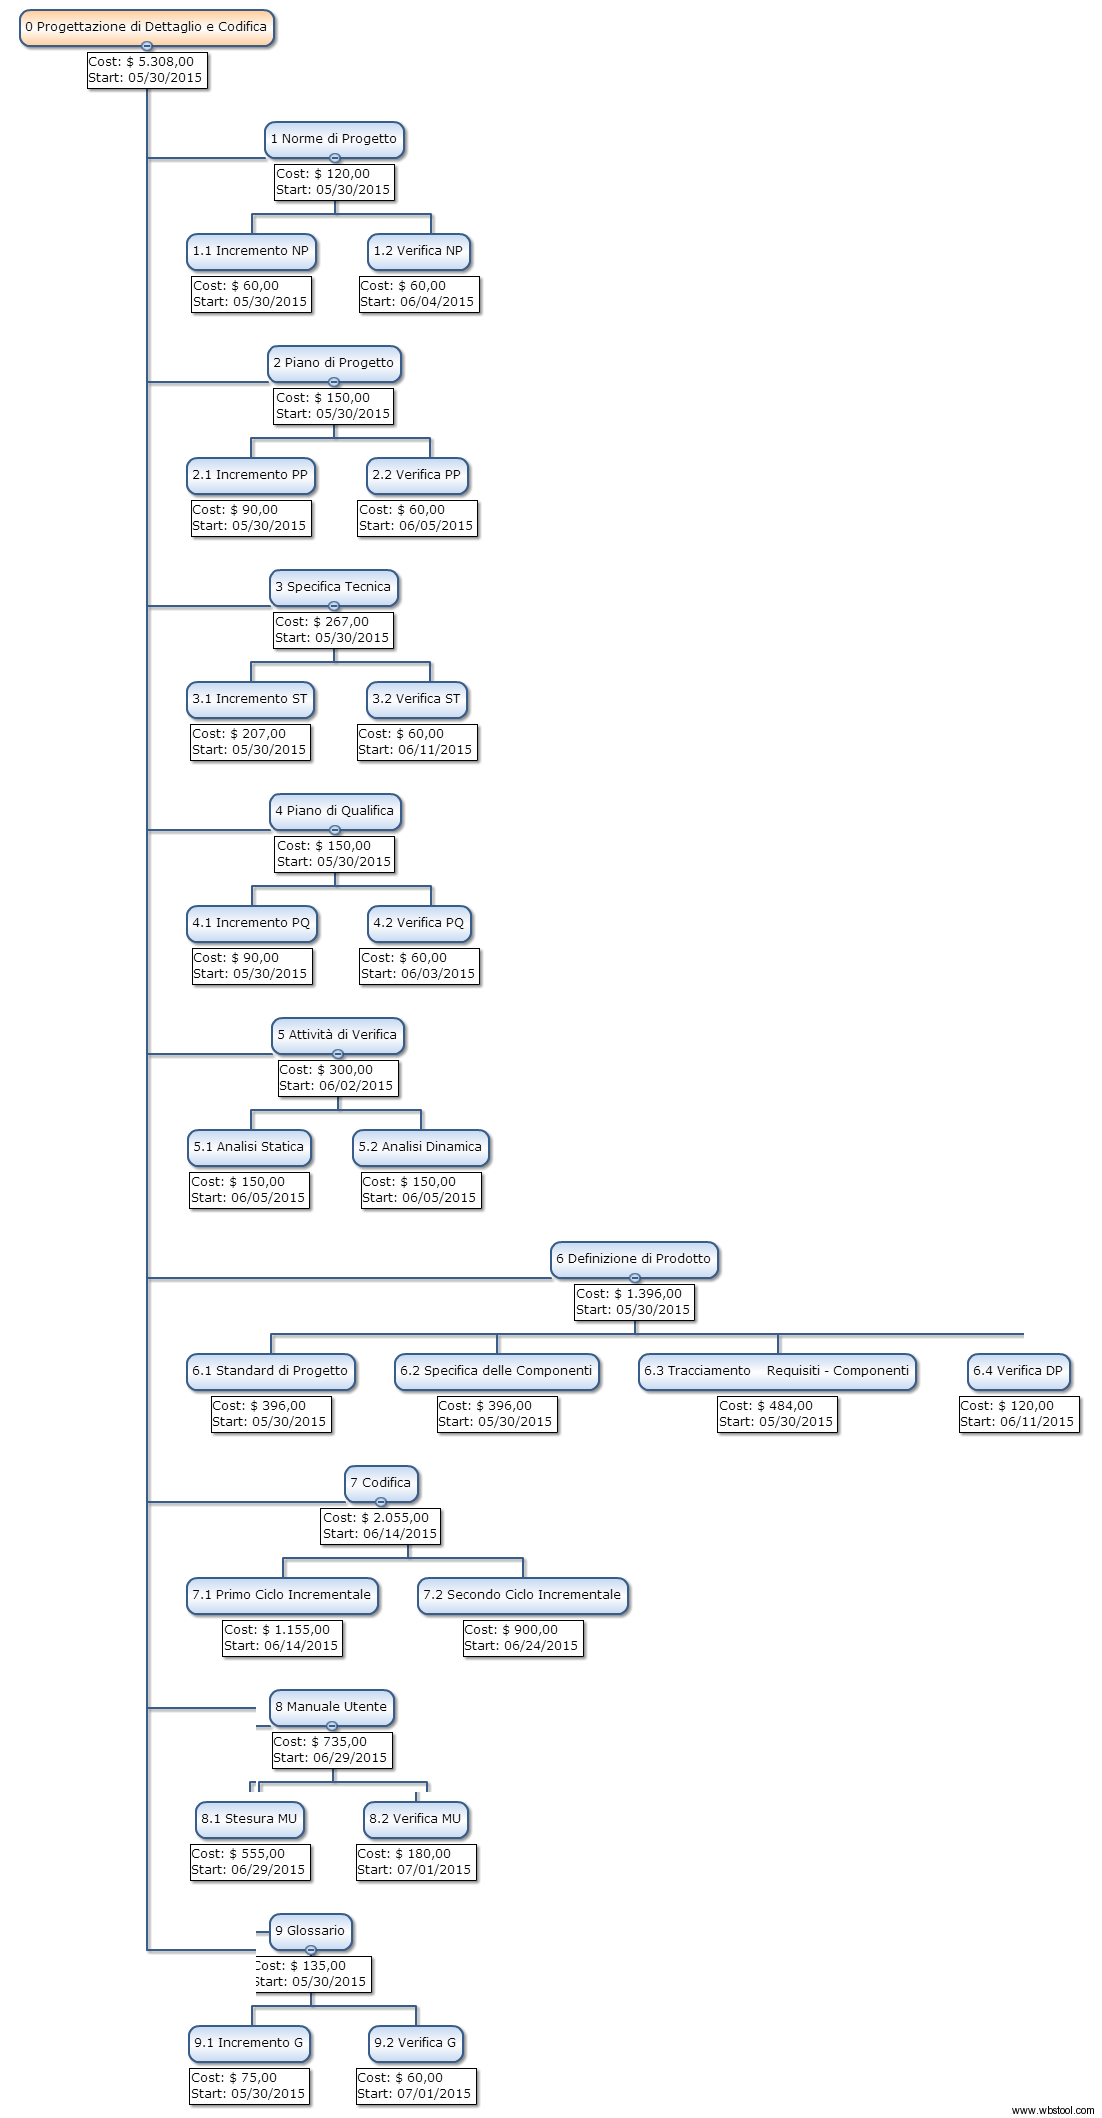
\includegraphics[width=0.5\textwidth]{./img/wbs_progettazione_dettaglio_codifica.png}
	\caption{Work Breakdown Structure, Progettazione di Dettaglio e Codifica}
\end{figure}

\newpage
\subsection{Verifica e Validazione}
\begin{description}
	\item[Periodo:] Dal 2015-06-19 al 2015-07-03 .
\end{description}
Questo periodo di lavoro ha inizio alla consegna della \textbf{Revisione di Qualifica} e ha termine con la consegna della \textbf{Revisione di Accettazione}, cioè col termine del processo dello sviluppo del software.

\noindent Le macro-attività principali sono:
\begin{itemize}
	\item \textbf{Validazione Verifica e Collaudo del Sistema:} il prodotto verrà convalidato per testare che è conforme alle specifiche e che soddisfa le richieste espresse dal cliente nel capitolato;
	\item \textbf{Incremento e Verifica:} verranno aggiornati ed incrementati tutti i documenti redatti sino ad ora in base ai risultati della \textit{Revisione di Qualifica}.
\end{itemize}
Si noti che non è da intendersi che le verifiche necessarie vengano fatte solamente durante \textbf{Verifica e Validazione}. Tale periodo incorpora le attività necessarie per il collaudo del prodotto. La verifica è un'attività presente in tutti i periodi precedenti e non è dunque da confondere con questo periodo.

\noindent I ruoli più utilizzati in questo periodo di lavoro sono: \textit{Progettista}, \textit{Programmatore} e \textit{Verificatore}.
\subsubsection{Diagramma di Gantt: Verifica e Validazione}
\begin{figure}[h] 
	\centering
	\includegraphics[width=\textwidth]{./img/verifica_validazione.png}
	\caption{Diagramma di Gantt, Verifica e Validazione}
\end{figure}

\newpage
\subsubsection{Work Breakdown Structure: Verifica e Validazione}
\begin{figure}[h]
	\centering
	\includegraphics[width=0.2\textwidth]{./img/wbs_verifica.png}
	\caption{Work Breakdown Structure, Verifica e Validazione}
\end{figure}


\newpage
\section{Suddivisione del lavoro}
I componenti del gruppo dovranno rivestire ciascuno, almeno una volta, tutti i ruoli di progetto indicati nella sezione 1.5 . Durante le varie fasi un componente può rivestire anche più ruoli contemporaneamente, purchè non si presentino casi di conflitti come, ad esempio, che una risorsa sia il verificatore di se stesso. 

\noindent Nelle sezioni successive si elencherà nel dettaglio la suddivisione del lavoro dei componenti nelle varie fasi di progetto.

\subsection{Analisi}
Nella fase di \textbf{Analisi} ciascun componente del gruppo dovrà rivestire i ruoli elencati nella seguente tabella:

\begin{table}[h]
\centering
\begin{tabular}{|l|c|c|c|c|c|c|c|}
\toprule
	\textbf{Cognome e Nome} & \multicolumn{6}{c}{\textbf{Ore per ruolo}} & \textbf{Ore Totali} \\
	& \textbf{Re} & \textbf{Am} & \textbf{An} & \textbf{Pt} & \textbf{Pr} & \textbf{Ve} & \\
	 
\midrule
	Agostinetto Matteo & 3 & & 16 & & & 3 & 22 \\
	Burlin Valerio & 14 & & & & & 8 & 22 \\ 
	Carraro Nicola & & & 16 & & & 6 & 22 \\
	Crespan Emanuele & & 14 & & & & 7 & 21 \\
	Ros Fabio & & & 18 & & & 3 & 21 \\
	Suierica Bogdan & & 12 & & & & 10 & 22 \\

\bottomrule
\end{tabular}
\caption{Ore a componente per ruolo, fase di Analisi}
\end{table}

I valori sono riassunti nel seguente grafico, che rappresenta in maniera visiva per quante ore un membro abbia ricoperto un determinato ruolo.

\subsection{Analisi di Dettaglio}
Nella fase di \textbf{Analisi di Dettaglio} ciascun componente del gruppo dovrà rivestire i ruoli elencati nella seguente tabella:

\begin{table}[h]
	\centering
	\begin{tabular}{|l|c|c|c|c|c|c|c|}
		\toprule
		\textbf{Cognome e Nome} & \multicolumn{6}{c}{\textbf{Ore per ruolo}} & \textbf{Ore Totali} \\
		& \textbf{Re} & \textbf{Am} & \textbf{An} & \textbf{Pt} & \textbf{Pr} & \textbf{Ve} & \\
		
		\midrule
		Agostinetto Matteo & & & & & & 6 & 6 \\
		Burlin Valerio & & & 6 & & & 2 & 8 \\ 
		Carraro Nicola & & 4 & & & & 2 & 6 \\
		Crespan Emanuele & & & 6 & & & & 6 \\
		Ros Fabio & 4 & & & & & 2 & 6 \\
		Suierica Bogdan & & & 6 & & & & 6 \\
		
		\bottomrule
	\end{tabular}
	\caption{Ore a componente per ruolo, fase di Analisi di Dettaglio}
\end{table}

I valori sono riassunti nel seguente grafico, che rappresenta in maniera visiva per quante ore un membro abbia ricoperto un determinato ruolo.

\subsection{Progettazione Architetturale}
Nella fase di \textbf{Progettazione Architetturale} ciascun componente del gruppo dovrà rivestire i ruoli elencati nella seguente tabella:

\begin{table}[h]
	\centering
	\begin{tabular}{|l|c|c|c|c|c|c|c|}
		\toprule
		\textbf{Cognome e Nome} & \multicolumn{6}{c}{\textbf{Ore per ruolo}} & \textbf{Ore Totali} \\
		& \textbf{Re} & \textbf{Am} & \textbf{An} & \textbf{Pt} & \textbf{Pr} & \textbf{Ve} & \\
		
		\midrule
		Agostinetto Matteo & & 5 & & 16 & & 7 & 28 \\
		Burlin Valerio & & & 8 & 16 & & 4 & 28 \\ 
		Carraro Nicola & 5 & & & 18 & & 5 & 28 \\
		Crespan Emanuele & & & & 18 & & 9 & 27 \\
		Ros Fabio & & & & 18 & & 9 & 27 \\
		Suierica Bogdan & & & 8 & 14 & & 7 & 29 \\
		
		\bottomrule
	\end{tabular}
	\caption{Ore a componente per ruolo, fase di Progettazione Architetturale}
\end{table}

I valori sono riassunti nel seguente grafico, che rappresenta in maniera visiva per quante ore un membro abbia ricoperto un determinato ruolo.

\subsection{Progettazione di Dettaglio e Codifica}
Nella fase di \textbf{Progettazione di Dettaglio e Codifica} ciascun componente del gruppo dovrà rivestire i ruoli elencati nella seguente tabella:

\begin{table}[h]
	\centering
	\begin{tabular}{|l|c|c|c|c|c|c|c|}
		\toprule
		\textbf{Cognome e Nome} & \multicolumn{6}{c}{\textbf{Ore per ruolo}} & \textbf{Ore Totali} \\
		& \textbf{Re} & \textbf{Am} & \textbf{An} & \textbf{Pt} & \textbf{Pr} & \textbf{Ve} & \\
		
		\midrule
		Agostinetto Matteo & & & & & 38 & 14 & 52 \\
		Burlin Valerio & & 4 & & 12 & 24 & 12 & 52 \\ 
		Carraro Nicola & & & & 4 & 32 & 16 & 52 \\
		Crespan Emanuele & & & 4 & 18 & 24 & 8 & 54 \\
		Ros Fabio & & & & 18 & 24 & 10 & 52 \\
		Suierica Bogdan & 4 & & & 12 & 32 & 6 & 54 \\
		
		\bottomrule
	\end{tabular}
	\caption{Ore a componente per ruolo, fase di Progettazione di Dettaglio e Codifica}
\end{table}

I valori sono riassunti nel seguente grafico, che rappresenta in maniera visiva per quante ore un membro abbia ricoperto un determinato ruolo.

\subsection{Verifica e Validazione}
Nella fase di \textbf{Verifica e Validazione} ciascun componente del gruppo dovrà rivestire i ruoli elencati nella seguente tabella:

\begin{table}[h]
	\centering
	\begin{tabular}{|l|c|c|c|c|c|c|c|}
		\toprule
		\textbf{Cognome e Nome} & \multicolumn{6}{c}{\textbf{Ore per ruolo}} & \textbf{Ore Totali} \\
		& \textbf{Re} & \textbf{Am} & \textbf{An} & \textbf{Pt} & \textbf{Pr} & \textbf{Ve} & \\
		
		\midrule
		Agostinetto Matteo & & & & 10 & & 15 & 25 \\
		Burlin Valerio & & & 8 & & 8 & 9 & 25 \\ 
		Carraro Nicola & & & & 10 & & 15 & 25 \\
		Crespan Emanuele & 8 & & & & & 16 & 24 \\
		Ros Fabio & & 8 & & & 8 & 10 & 26 \\
		Suierica Bogdan & & & & 5 & & 17 & 22 \\
		
		\bottomrule
	\end{tabular}
	\caption{Ore a componente per ruolo, fase di Verifica e Validazione}
\end{table}

I valori sono riassunti nel seguente grafico, che rappresenta in maniera visiva per quante ore un membro abbia ricoperto un determinato ruolo.

\subsection{Totale}
La seguente tabella illustra le ore totali che ogni componente del gruppo dedicherà al progetto, mettendo in evidenza anche le ore che verranno poi rendicontate.

\begin{table}[h]
	\centering
	\begin{tabular}{|l|l|c|c|c|c|c|c|c|}
		\toprule
		\textbf{Cognome e Nome} & \multicolumn{7}{c}{\textbf{Ore per ruolo}} & \textbf{Ore Totali} \\
		& & \textbf{Re} & \textbf{Am} & \textbf{An} & \textbf{Pt} & \textbf{Pr} & \textbf{Ve} & \\
		
		\midrule
		\multirow{2}*{Agostinetto Matteo} & Totale & 3 & 5 & 16 & 26 & 38 & 45 & 133 \\
										  & Rendicontate & & 5 & & 26 & 38 & 36 & 105 \\
		\midrule
		\multirow{2}*{Burlin Valerio} & Totale & 14 & 4 & 22 & 28 & 32 & 35 & 135 \\
		                              & Rendicontate & 0 & 4 & 16 & 28 & 32 & 25 & 105 \\ 
		\midrule
		\multirow{2}*{Carraro Nicola} & Totale & 5 & 4 & 16 & 32 & 32 & 44 & 133 \\
		                              & Rendicontate & 5 & & & 32 & 32 & 46 & 105 \\
		\midrule
		\multirow{2}*{Crespan Emanuele} & Totale & 8 & 14 & 10 & 36 & 24 & 40 & 132 \\
		                                & Rendicontate & 8 & & 4 & 36 & 24 & 33 & 105 \\
		\midrule                                
		\multirow{2}*{Ros Fabio} & Totale & 4 & 8 & 18 & 36 & 32 & 34 & 132 \\
		                         & Rendicontate & 0 & 8 & 0 & 36 & 32 & 29 & 105 \\ 
		\midrule                         
		\multirow{2}*{Suierica Bogdan} & Totale & 4 & 12 & 14 & 31 & 32 & 40 & 133 \\
		                               & Rendicontate & 4 & & 8 & 31 & 32 & 30 & 105 \\
		
		\bottomrule
	\end{tabular}
	\caption{Ore a componente per ruolo, Totali e Rendicontate}
	\label{tab1}
\end{table}

I valori sono riassunti nei seguenti grafici che visualizzano le ore che un membro ha ricoperto in un determinato ruolo, sia le ore totali che quelle rendicontate.
\newpage
\section{Prospetto economico}
In questa sezione vengono presentati, per ogni macro-fase di progetto, le ore preventivate di impiego per i ruoli coinvolti.

\noindent Occorre ricordare che le macro-fasi di \textbf{Analisi} e \textbf{Analisi di Dettaglio} non sono a carico del committente e quindi non saranno considerate nel computo delle ore totali da retribuire, ma verranno riportate ugualmente per dare un'immagine di insieme.

\subsection{Analisi}
In questa macro-fase, le ore ripartite tra i ruoli ed i conseguenti costi sono evidenziati dalla seguente tabella:

\begin{table}[h]
\centering
\begin{tabular}{|l|c|c|}
	\toprule
	\textbf{Ruolo} & \textbf{Ore per ruolo} & \textbf{Costo per ruolo} \\
			
	\midrule
	Responsabile di Progetto & 17 & 510 \\
	Amministratore di Progetto & 26 & 520 \\ 
	Analista & 50 & 1250 \\
	Progettista & & \\
	Programmatore & & \\
	Verificatore & 37 & 555 \\
	\midrule
	\textbf{Totale} & 130 & 2835 \\
				
	\bottomrule
\end{tabular}
\caption{Costo per ruolo, Analisi}
\end{table}

\noindent Il seguente grafico illustra come ciascun ruolo abbia influito sul totale delle ore di questa macro-fase:

\def\angle{0}
\def\radius{3}
\def\cyclelist{{"blue","red","yellow","green"}}
\newcount\cyclecount \cyclecount=-1
\newcount\ind \ind=-1
\begin{figure}[h]
\centering
\begin{tikzpicture}[nodes = {font=\sffamily}]
\foreach \percent/\name in {
	13/Responsabile di Progetto,
	20/Amministratore di Progetto,
	39/Analista,
	28/Verificatore
} {
\ifx\percent\empty\else               % If \percent is empty, do nothing
\global\advance\cyclecount by 1     % Advance cyclecount
\global\advance\ind by 1            % Advance list index
\ifnum3<\cyclecount                 % If cyclecount is larger than list
\global\cyclecount=0              %   reset cyclecount and
\global\ind=0                     %   reset list index
\fi
\pgfmathparse{\cyclelist[\the\ind]} % Get color from cycle list
\edef\color{\pgfmathresult}         %   and store as \color
% Draw angle and set labels
\draw[fill={\color!50},draw={\color}] (0,0) -- (\angle:\radius)
arc (\angle:\angle+\percent*3.6:\radius) -- cycle;
\node at (\angle+0.5*\percent*3.6:0.7*\radius) {\percent\,\%};
\node[pin=\angle+0.5*\percent*3.6:\name]
at (\angle+0.5*\percent*3.6:\radius) {};
\pgfmathparse{\angle+\percent*3.6}  % Advance angle
\xdef\angle{\pgfmathresult}         %   and store in \angle
\fi
};
\end{tikzpicture}
\caption{Ore per ruoli, Analisi}
\end{figure}
\newpage

\noindent Il seguente grafico illustra come ciascun ruolo abbia influito sul totale dei costi di questa macro-fase:

\begin{figure}[h]
\centering
\begin{tikzpicture}[nodes = {font=\sffamily}]
	\foreach \percent/\name in {
		18/Responsabile di Progetto,
		18/Amministratore di Progetto,
		44/Analista,
		20/Verificatore
	} {
		\ifx\percent\empty\else               % If \percent is empty, do nothing
		\global\advance\cyclecount by 1     % Advance cyclecount
		\global\advance\ind by 1            % Advance list index
		\ifnum3<\cyclecount                 % If cyclecount is larger than list
		\global\cyclecount=0              %   reset cyclecount and
		\global\ind=0                     %   reset list index
		\fi
		\pgfmathparse{\cyclelist[\the\ind]} % Get color from cycle list
		\edef\color{\pgfmathresult}         %   and store as \color
		% Draw angle and set labels
		\draw[fill={\color!50},draw={\color}] (0,0) -- (\angle:\radius)
		arc (\angle:\angle+\percent*3.6:\radius) -- cycle;
		\node at (\angle+0.5*\percent*3.6:0.7*\radius) {\percent\,\%};
		\node[pin=\angle+0.5*\percent*3.6:\name]
		at (\angle+0.5*\percent*3.6:\radius) {};
		\pgfmathparse{\angle+\percent*3.6}  % Advance angle
		\xdef\angle{\pgfmathresult}         %   and store in \angle
		\fi
	};
\end{tikzpicture}
\caption{Costo per ruoli, Analisi}
\end{figure}

\subsection{Analisi di Dettaglio}
In questa macro-fase, le ore ripartite tra i ruoli ed i conseguenti costi sono evidenziati dalla seguente tabella:

\begin{table}[h]
\centering
\begin{tabular}{|l|c|c|}
	\toprule
	\textbf{Ruolo} & \textbf{Ore per ruolo} & \textbf{Costo per ruolo} \\
		
	\midrule
	Responsabile di Progetto & 4 & 120 \\
	Amministratore di Progetto & 4 & 80 \\ 
	Analista & 18 & 450 \\
	Progettista & & \\
	Programmatore & & \\
	Verificatore & 12 & 180 \\
	\midrule
	\textbf{Totale} & 38 & 830 \\
		
	\bottomrule
\end{tabular}
\caption{Costo per ruolo, Analisi di Dettaglio}
\end{table}

\newpage
\noindent I seguenti grafici illustrano rispettivamente come ciascun ruolo abbia influito sul totale delle ore e dei costi di questa macro-fase:

\begin{figure}[h]
\centering
\begin{tikzpicture}[nodes = {font=\sffamily}]
	\foreach \percent/\name in {
		11/Responsabile di Progetto,
		11/Amministratore di Progetto,
		47/Analista,
		31/Verificatore
	} {
	\ifx\percent\empty\else               % If \percent is empty, do nothing
	\global\advance\cyclecount by 1     % Advance cyclecount
	\global\advance\ind by 1            % Advance list index
	\ifnum3<\cyclecount                 % If cyclecount is larger than list
	\global\cyclecount=0              %   reset cyclecount and
	\global\ind=0                     %   reset list index
	\fi
	\pgfmathparse{\cyclelist[\the\ind]} % Get color from cycle list
	\edef\color{\pgfmathresult}         %   and store as \color
	% Draw angle and set labels
	\draw[fill={\color!50},draw={\color}] (0,0) -- (\angle:\radius)
	arc (\angle:\angle+\percent*3.6:\radius) -- cycle;
	\node at (\angle+0.5*\percent*3.6:0.7*\radius) {\percent\,\%};
	\node[pin=\angle+0.5*\percent*3.6:\name]
	at (\angle+0.5*\percent*3.6:\radius) {};
	\pgfmathparse{\angle+\percent*3.6}  % Advance angle
	\xdef\angle{\pgfmathresult}         %   and store in \angle
	\fi
};
\end{tikzpicture}
\caption{Ore per ruoli, Analisi di Dettaglio}
\end{figure}

\begin{figure}[h]
\centering
\begin{tikzpicture}[nodes = {font=\sffamily}]
	\foreach \percent/\name in {
		14/Responsabile di Progetto,
		10/Amministratore di Progetto,
		54/Analista,
		22/Verificatore
	} {
	\ifx\percent\empty\else               % If \percent is empty, do nothing
	\global\advance\cyclecount by 1     % Advance cyclecount
	\global\advance\ind by 1            % Advance list index
	\ifnum3<\cyclecount                 % If cyclecount is larger than list
	\global\cyclecount=0              %   reset cyclecount and
	\global\ind=0                     %   reset list index
	\fi
	\pgfmathparse{\cyclelist[\the\ind]} % Get color from cycle list
	\edef\color{\pgfmathresult}         %   and store as \color
	% Draw angle and set labels
	\draw[fill={\color!50},draw={\color}] (0,0) -- (\angle:\radius)
	arc (\angle:\angle+\percent*3.6:\radius) -- cycle;
	\node at (\angle+0.5*\percent*3.6:0.7*\radius) {\percent\,\%};
	\node[pin=\angle+0.5*\percent*3.6:\name]
	at (\angle+0.5*\percent*3.6:\radius) {};
	\pgfmathparse{\angle+\percent*3.6}  % Advance angle
	\xdef\angle{\pgfmathresult}         %   and store in \angle
	\fi
};
\end{tikzpicture}
\caption{Costo per ruoli, Analisi di Dettaglio}
\end{figure}
\newpage
\subsection{Progettazione Architetturale}
In questa macro-fase, le ore ripartite tra i ruoli ed i conseguenti costi sono evidenziati dalla seguente tabella:

\begin{table}[h]
\centering
\begin{tabular}{|l|c|c|}
	\toprule
	\textbf{Ruolo} & \textbf{Ore per ruolo} & \textbf{Costo per ruolo} \\
		
	\midrule
	Responsabile di Progetto & 5 & 150 \\
	Amministratore di Progetto & 5 & 100 \\ 
	Analista & 16 & 400 \\
	Progettista & 100 & 2200 \\
	Programmatore & & \\
	Verificatore & 41 & 615 \\
	\midrule
	\textbf{Totale} & 167 & 3465 \\
	
	\bottomrule
\end{tabular}
\caption{Costo per ruolo, Progettazione Architetturale}
\end{table}

\noindent Il seguente grafico illustra come ciascun ruolo abbia influito sul totale delle ore di questa macro-fase:

\def\cyclelist{{"red","yellow","magenta","green","blue"}}
\begin{figure}[h]
\centering
\begin{tikzpicture}[nodes = {font=\sffamily}]
	\foreach \percent/\name in {
		3/Responsabile di Progetto,
		3/Amministratore di Progetto,
		10/Analista,
		60/Progettista,
		24/Verificatore
	} {
	\ifx\percent\empty\else               % If \percent is empty, do nothing
	\global\advance\cyclecount by 1     % Advance cyclecount
	\global\advance\ind by 1            % Advance list index
	\ifnum4<\cyclecount                 % If cyclecount is larger than list
	\global\cyclecount=0              %   reset cyclecount and
	\global\ind=0                     %   reset list index
	\fi
	\pgfmathparse{\cyclelist[\the\ind]} % Get color from cycle list
	\edef\color{\pgfmathresult}         %   and store as \color
	% Draw angle and set labels
	\draw[fill={\color!50},draw={\color}] (0,0) -- (\angle:\radius)
	arc (\angle:\angle+\percent*3.6:\radius) -- cycle;
	\node at (\angle+0.5*\percent*3.6:0.7*\radius) {\percent\,\%};
	\node[pin=\angle+0.5*\percent*3.6:\name]
	at (\angle+0.5*\percent*3.6:\radius) {};
	\pgfmathparse{\angle+\percent*3.6}  % Advance angle
	\xdef\angle{\pgfmathresult}         %   and store in \angle
	\fi
};
\end{tikzpicture}
\caption{Ore per ruoli, Progettazione Architetturale}
\end{figure}
\newpage

\noindent Il seguente grafico illustra come ciascun ruolo abbia influito sul totale dei costi di questa macro-fase:

\begin{figure}[h]
\centering
\begin{tikzpicture}[nodes = {font=\sffamily}]
	\foreach \percent/\name in {
		4/Responsabile di Progetto,
		3/Amministratore di Progetto,
		12/Analista,
		63/Progettista,
		18/Verificatore
	} {
	\ifx\percent\empty\else               % If \percent is empty, do nothing
	\global\advance\cyclecount by 1     % Advance cyclecount
	\global\advance\ind by 1            % Advance list index
	\ifnum4<\cyclecount                 % If cyclecount is larger than list
	\global\cyclecount=0              %   reset cyclecount and
	\global\ind=0                     %   reset list index
	\fi
	\pgfmathparse{\cyclelist[\the\ind]} % Get color from cycle list
	\edef\color{\pgfmathresult}         %   and store as \color
	% Draw angle and set labels
	\draw[fill={\color!50},draw={\color}] (0,0) -- (\angle:\radius)
	arc (\angle:\angle+\percent*3.6:\radius) -- cycle;
	\node at (\angle+0.5*\percent*3.6:0.7*\radius) {\percent\,\%};
	\node[pin=\angle+0.5*\percent*3.6:\name]
	at (\angle+0.5*\percent*3.6:\radius) {};
	\pgfmathparse{\angle+\percent*3.6}  % Advance angle
	\xdef\angle{\pgfmathresult}         %   and store in \angle
	\fi
};
\end{tikzpicture}
\caption{Costo per ruoli, Progettazione Architetturale}
\end{figure}

\subsection{Progettazione di Dettaglio e Codifica}
In questa macro-fase, le ore ripartite tra i ruoli ed i conseguenti costi sono evidenziati dalla seguente tabella:

\begin{table}[h]
\centering
\begin{tabular}{|l|c|c|}
	\toprule
	\textbf{Ruolo} & \textbf{Ore per ruolo} & \textbf{Costo per ruolo} \\
		
	\midrule
	Responsabile di Progetto & 4 & 120 \\
	Amministratore di Progetto & 4 & 80 \\ 
	Analista & 4 & 100 \\
	Progettista & 64 & 1408 \\
	Programmatore & 174 & 2610 \\
	Verificatore & 66 & 990 \\
	\midrule
	\textbf{Totale} & 316 & 5308 \\
	
	\bottomrule
\end{tabular}
\caption{Costo per ruolo, Progettazione di Dettaglio e Codifica}
\end{table}

\newpage
\noindent I seguenti grafici illustrano rispettivamente come ciascun ruolo abbia influito sul totale delle ore e dei costi di questa macro-fase:
\def\cyclelist{{"yellow","magenta","orange","green","blue","red"}}
\begin{figure}[h]
\centering
\begin{tikzpicture}[nodes = {font=\sffamily}]
	\foreach \percent/\name in {
		1/Responsabile di Progetto,
		1/Amministratore di Progetto,
		1/Analista,
		21/Progettista,
		55/Programmatore,
		21/Verificatore
	} {
	\ifx\percent\empty\else               % If \percent is empty, do nothing
	\global\advance\cyclecount by 1     % Advance cyclecount
	\global\advance\ind by 1            % Advance list index
	\ifnum5<\cyclecount                 % If cyclecount is larger than list
	\global\cyclecount=0              %   reset cyclecount and
	\global\ind=0                     %   reset list index
	\fi
	\pgfmathparse{\cyclelist[\the\ind]} % Get color from cycle list
	\edef\color{\pgfmathresult}         %   and store as \color
	% Draw angle and set labels
	\draw[fill={\color!50},draw={\color}] (0,0) -- (\angle:\radius)
	arc (\angle:\angle+\percent*3.6:\radius) -- cycle;
	\node at (\angle+0.5*\percent*3.6:0.7*\radius) {\percent\,\%};
	\node[pin=\angle+0.5*\percent*3.6:\name]
	at (\angle+0.5*\percent*3.6:\radius) {};
	\pgfmathparse{\angle+\percent*3.6}  % Advance angle
	\xdef\angle{\pgfmathresult}         %   and store in \angle
	\fi
};
\end{tikzpicture}
\caption{Ore per ruoli, Progettazione di Dettaglio e Codifica}
\end{figure}

\begin{figure}[h]
\centering
\begin{tikzpicture}[nodes = {font=\sffamily}]
	\foreach \percent/\name in {
		2/Responsabile di Progetto,
		1/Amministratore di Progetto,
		2/Analista,
		27/Progettista,
		49/Programmatore,
		19/Verificatore
	} {
	\ifx\percent\empty\else               % If \percent is empty, do nothing
	\global\advance\cyclecount by 1     % Advance cyclecount
	\global\advance\ind by 1            % Advance list index
	\ifnum5<\cyclecount                 % If cyclecount is larger than list
	\global\cyclecount=0              %   reset cyclecount and
	\global\ind=0                     %   reset list index
	\fi
	\pgfmathparse{\cyclelist[\the\ind]} % Get color from cycle list
	\edef\color{\pgfmathresult}         %   and store as \color
	% Draw angle and set labels
	\draw[fill={\color!50},draw={\color}] (0,0) -- (\angle:\radius)
	arc (\angle:\angle+\percent*3.6:\radius) -- cycle;
	\node at (\angle+0.5*\percent*3.6:0.7*\radius) {\percent\,\%};
	\node[pin=\angle+0.5*\percent*3.6:\name]
	at (\angle+0.5*\percent*3.6:\radius) {};
	\pgfmathparse{\angle+\percent*3.6}  % Advance angle
	\xdef\angle{\pgfmathresult}         %   and store in \angle
	\fi
};
\end{tikzpicture}
\caption{Costo per ruoli, Progettazione di Dettaglio e Codifica}
\end{figure}

\newpage
\subsection{Verifica e Validazione}
In questa macro-fase, le ore ripartite tra i ruoli ed i conseguenti costi sono evidenziati dalla seguente tabella:

\begin{table}[h]
\centering
\begin{tabular}{|l|c|c|}
	\toprule
	\textbf{Ruolo} & \textbf{Ore per ruolo} & \textbf{Costo per ruolo} \\
		
	\midrule
	Responsabile di Progetto & 8 & 240 \\
	Amministratore di Progetto & 8 & 160 \\ 
	Analista & 8 & 200 \\
	Progettista & 25 & 550 \\
	Programmatore & 16 & 240 \\
	Verificatore & 82 & 1230 \\
	\midrule
	\textbf{Totale} & 147 & 2620 \\
		
	\bottomrule
\end{tabular}
\caption{Costo per ruolo, Verifica e Validazione}
\end{table}

\noindent Il seguente grafico illustra come ciascun ruolo abbia influito sul totale delle ore di questa macro-fase:

\begin{figure}[h]
\centering
\begin{tikzpicture}[nodes = {font=\sffamily}]
	\foreach \percent/\name in {
		6/Responsabile di Progetto,
		6/Amministratore di Progetto,
		6/Analista,
		17/Progettista,
		10/Programmatore,
		55/Verificatore
	} {
	\ifx\percent\empty\else               % If \percent is empty, do nothing
	\global\advance\cyclecount by 1     % Advance cyclecount
	\global\advance\ind by 1            % Advance list index
	\ifnum5<\cyclecount                 % If cyclecount is larger than list
	\global\cyclecount=0              %   reset cyclecount and
	\global\ind=0                     %   reset list index
	\fi
	\pgfmathparse{\cyclelist[\the\ind]} % Get color from cycle list
	\edef\color{\pgfmathresult}         %   and store as \color
	% Draw angle and set labels
	\draw[fill={\color!50},draw={\color}] (0,0) -- (\angle:\radius)
	arc (\angle:\angle+\percent*3.6:\radius) -- cycle;
	\node at (\angle+0.5*\percent*3.6:0.7*\radius) {\percent\,\%};
	\node[pin=\angle+0.5*\percent*3.6:\name]
	at (\angle+0.5*\percent*3.6:\radius) {};
	\pgfmathparse{\angle+\percent*3.6}  % Advance angle
	\xdef\angle{\pgfmathresult}         %   and store in \angle
	\fi
};
\end{tikzpicture}
\caption{Ore per ruoli, Verifica e Validazione}
\end{figure}

\newpage
\noindent Il seguente grafico illustra come ciascun ruolo abbia influito sul totale dei costi di questa macro-fase:

\begin{figure}[h]
\centering
\begin{tikzpicture}[nodes = {font=\sffamily}]
	\foreach \percent/\name in {
		9/Responsabile di Progetto,
		6/Amministratore di Progetto,
		8/Analista,
		21/Progettista,
		9/Programmatore,
		47/Verificatore
	} {
	\ifx\percent\empty\else               % If \percent is empty, do nothing
	\global\advance\cyclecount by 1     % Advance cyclecount
	\global\advance\ind by 1            % Advance list index
	\ifnum5<\cyclecount                 % If cyclecount is larger than list
	\global\cyclecount=0              %   reset cyclecount and
	\global\ind=0                     %   reset list index
	\fi
	\pgfmathparse{\cyclelist[\the\ind]} % Get color from cycle list
	\edef\color{\pgfmathresult}         %   and store as \color
	% Draw angle and set labels
	\draw[fill={\color!50},draw={\color}] (0,0) -- (\angle:\radius)
	arc (\angle:\angle+\percent*3.6:\radius) -- cycle;
	\node at (\angle+0.5*\percent*3.6:0.7*\radius) {\percent\,\%};
	\node[pin=\angle+0.5*\percent*3.6:\name]
	at (\angle+0.5*\percent*3.6:\radius) {};
	\pgfmathparse{\angle+\percent*3.6}  % Advance angle
	\xdef\angle{\pgfmathresult}         %   and store in \angle
	\fi
};
\end{tikzpicture}
\caption{Costo per ruoli, Verifica e Validazione}
\end{figure}

\subsection{Totale}
\subsubsection{Ore totali e rendicontate}
Le ore totali previste per la realizzazione dell'intero progetto, suddivise in ore totali e rendicontate, ed i conseguenti costi sono riportate nella seguente tabella:

\begin{table}[h]
\centering
\begin{tabular}{|l|l|c|c|c|c|c|c|c|}
	\toprule
	\textbf{Ruolo} & & \textbf{Ore per ruolo} & \textbf{Costo per ruolo} \\
		
	\midrule
	\multirow{2}*{Responsabile di Progetto} & Totale & 38 & 1140 \\
												& Rendicontanto & 17 & 510 \\
    \midrule
	\multirow{2}*{Amministratore di Progetto} & Totale & 47 & 940 \\
												  & Rendicontanto & 17 & 340 \\ 
	\midrule
	\multirow{2}*{Analista} & Totale & 96 & 2400 \\
								& Rendicontanto & 28 & 700 \\
	\midrule
	\multirow{2}*{Progettista} & Totale & 189 & 4158 \\
								   & Rendicontanto & 189 & 4158 \\
	\midrule
	\multirow{2}*{Programmatore} & Totale & 190 & 2850 \\
									 & Rendicontanto & 190 & 2850 \\ 
	\midrule
	\multirow{2}*{Verificatore} & Totale & 238 & 3570 \\
									& Rendicontanto & 189 & 2835 \\
	\midrule							
	\multirow{2}*{} & Totale & 798 & 15058 \\
						& Rendicontanto & \textbf{630} & \textbf{11393} \\
	\bottomrule
		
\end{tabular}
\caption{Ore a componente per ruolo, Totali e Rendicontate}
\label{tab2}
\end{table}

\newpage
\noindent I seguenti grafici illustrano, rispettivamente, l'incidenza di ciascun ruolo su orari e costi totali del progetto \PROGETTO:

\begin{figure}[h]
\centering
\begin{tikzpicture}[nodes = {font=\sffamily}]
	\foreach \percent/\name in {
		5/Responsabile di Progetto,
		6/Amministratore di Progetto,
		12/Analista,
		23/Progettista,
		24/Programmatore,
		30/Verificatore
	} {
	\ifx\percent\empty\else               % If \percent is empty, do nothing
	\global\advance\cyclecount by 1     % Advance cyclecount
	\global\advance\ind by 1            % Advance list index
	\ifnum5<\cyclecount                 % If cyclecount is larger than list
	\global\cyclecount=0              %   reset cyclecount and
	\global\ind=0                     %   reset list index
	\fi
	\pgfmathparse{\cyclelist[\the\ind]} % Get color from cycle list
	\edef\color{\pgfmathresult}         %   and store as \color
	% Draw angle and set labels
	\draw[fill={\color!50},draw={\color}] (0,0) -- (\angle:\radius)
	arc (\angle:\angle+\percent*3.6:\radius) -- cycle;
	\node at (\angle+0.5*\percent*3.6:0.7*\radius) {\percent\,\%};
	\node[pin=\angle+0.5*\percent*3.6:\name]
	at (\angle+0.5*\percent*3.6:\radius) {};
	\pgfmathparse{\angle+\percent*3.6}  % Advance angle
	\xdef\angle{\pgfmathresult}         %   and store in \angle
	\fi
};
\end{tikzpicture}
\caption{Ore totali per ruoli}
\end{figure}

\begin{figure}[h]
\centering
\begin{tikzpicture}[nodes = {font=\sffamily}]
	\foreach \percent/\name in {
		7/Responsabile di Progetto,
		6/Amministratore di Progetto,
		16/Analista,
		28/Progettista,
		19/Programmatore,
		24/Verificatore
	} {
	\ifx\percent\empty\else               % If \percent is empty, do nothing
	\global\advance\cyclecount by 1     % Advance cyclecount
	\global\advance\ind by 1            % Advance list index
	\ifnum5<\cyclecount                 % If cyclecount is larger than list
	\global\cyclecount=0              %   reset cyclecount and
	\global\ind=0                     %   reset list index
	\fi
	\pgfmathparse{\cyclelist[\the\ind]} % Get color from cycle list
	\edef\color{\pgfmathresult}         %   and store as \color
	% Draw angle and set labels
	\draw[fill={\color!50},draw={\color}] (0,0) -- (\angle:\radius)
	arc (\angle:\angle+\percent*3.6:\radius) -- cycle;
	\node at (\angle+0.5*\percent*3.6:0.7*\radius) {\percent\,\%};
	\node[pin=\angle+0.5*\percent*3.6:\name]
	at (\angle+0.5*\percent*3.6:\radius) {};
	\pgfmathparse{\angle+\percent*3.6}  % Advance angle
	\xdef\angle{\pgfmathresult}         %   and store in \angle
	\fi
};
\end{tikzpicture}
\caption{Costi totali per ruoli}
\end{figure}

\newpage
\noindent I seguenti grafici illustrano, rispettivamente, l'incidenza di ciascun ruolo su orari e costi rendicontati del progetto \PROGETTO:

\begin{figure}[h]
\centering
\begin{tikzpicture}[nodes = {font=\sffamily}]
	\foreach \percent/\name in {
		3/Responsabile di Progetto,
		3/Amministratore di Progetto,
		4/Analista,
		30/Progettista,
		30/Programmatore,
		30/Verificatore
	} {
	\ifx\percent\empty\else               % If \percent is empty, do nothing
	\global\advance\cyclecount by 1     % Advance cyclecount
	\global\advance\ind by 1            % Advance list index
	\ifnum5<\cyclecount                 % If cyclecount is larger than list
	\global\cyclecount=0              %   reset cyclecount and
	\global\ind=0                     %   reset list index
	\fi
	\pgfmathparse{\cyclelist[\the\ind]} % Get color from cycle list
	\edef\color{\pgfmathresult}         %   and store as \color
	% Draw angle and set labels
	\draw[fill={\color!50},draw={\color}] (0,0) -- (\angle:\radius)
	arc (\angle:\angle+\percent*3.6:\radius) -- cycle;
	\node at (\angle+0.5*\percent*3.6:0.7*\radius) {\percent\,\%};
	\node[pin=\angle+0.5*\percent*3.6:\name]
	at (\angle+0.5*\percent*3.6:\radius) {};
	\pgfmathparse{\angle+\percent*3.6}  % Advance angle
	\xdef\angle{\pgfmathresult}         %   and store in \angle
	\fi
};
\end{tikzpicture}
\caption{Ore rendicontate per ruoli}
\end{figure}

\begin{figure}[h]
\centering
\begin{tikzpicture}[nodes = {font=\sffamily}]
	\foreach \percent/\name in {
		4/Responsabile di Progetto,
		3/Amministratore di Progetto,
		6/Analista,
		37/Progettista,
		25/Programmatore,
		25/Verificatore
	} {
	\ifx\percent\empty\else               % If \percent is empty, do nothing
	\global\advance\cyclecount by 1     % Advance cyclecount
	\global\advance\ind by 1            % Advance list index
	\ifnum5<\cyclecount                 % If cyclecount is larger than list
	\global\cyclecount=0              %   reset cyclecount and
	\global\ind=0                     %   reset list index
	\fi
	\pgfmathparse{\cyclelist[\the\ind]} % Get color from cycle list
	\edef\color{\pgfmathresult}         %   and store as \color
	% Draw angle and set labels
	\draw[fill={\color!50},draw={\color}] (0,0) -- (\angle:\radius)
	arc (\angle:\angle+\percent*3.6:\radius) -- cycle;
	\node at (\angle+0.5*\percent*3.6:0.7*\radius) {\percent\,\%};
	\node[pin=\angle+0.5*\percent*3.6:\name]
	at (\angle+0.5*\percent*3.6:\radius) {};
	\pgfmathparse{\angle+\percent*3.6}  % Advance angle
	\xdef\angle{\pgfmathresult}         %   and store in \angle
	\fi
};
\end{tikzpicture}
\caption{Costi rendicontati per ruoli}
\end{figure}

\subsubsection{Conclusioni}
Il costo totale per realizzare \PROGETTO{} evidenziato in tabella~\ref{tab2} e imputabile al proponente è di 11393 euro. Tale progetto richiede 630 ore di sviluppo ovvero un totale di ore 105 a componente, come illustrato precedentemente nella tabella~\ref{tab1}.


\newpage
\section{Analisi dei rischi}
Al fine di migliorare l'andamento del progetto si è effettuata un'attenta analisi dei rischi. Essa è suddivisa in quattro fasi:
\begin{itemize}
	\item \textbf{Identificazione:} individuare i rischi che possono interessare il progetto, indicandone le cause e cercando di prevederne
	le conseguenze. I rischi possono riguardare:
	\begin{itemize}
		\item \textbf{Progetto:} relativi a pianificazione, risorse e strumenti;
		\item \textbf{Prodotto:} relativi a conformità alle aspettative del committente;
		\item \textbf{\gls{Business}:} relativi a costi e concorrenza sul mercato.
	\end{itemize}
	\item \textbf{Analisi:} prevedere le probabilità di occorrenza del rischio e determinare le possibili conseguenze;
	\item \textbf{Pianificazione:} ideare una strategia per prevenire i possibili rischi;
	\item \textbf{Monitoraggio:} elaborare metodi di verifica e controllo per riconoscere anticipatamente i rischi, per il loro trattamento e la loro mitigazione.
\end{itemize}
Ogni rischio identificato è descritto con: nome, probabilità di occorrenza del rischio, livello di pericolosità, descrizione strategie per la rilevazione e contromisure. Ciascun rischio verrà monitorato nel tempo e ne verrà descritto l'effettivo riscontro con l'avanzare del progetto.

\subsection{Livello tecnologico}
\subsubsection{Tecnologie adottate}
\begin{description}
	\item[Livello di rischio:] medio.
	\item[Probabilità:] bassa.
	\item[Descrizione:] le tecnologie richieste dal capitolato sono \gls{HTML5}, \gls{Javascript} e \gls{CSS}. Tali linguaggi sono noti a tutto il gruppo in quanto progetti didattici svolti in anni passati ne richiedevano la conoscenza. Non è da escludere che si possano incontrare difficoltà per alcuni particolari requisiti da soddisfare e per l'utilizzo di \gls{framework} totalmente sconosciuti come \textit{\gls{Reveal.js}} e \textit{\gls{Angular.js}}.
	\item[Identificazione:] sarà compito del \textit{Responsabile di Progetto} monitorare costantemente il grado di conoscenza dei membri del gruppo riguardo le tecnologie che si andranno ad utilizzare.
	\item[Gestione:] per evitare di incorrere in gravi ritardi, ogni membro del gruppo ha il compito di studiare ed approfondire la propria conoscenza delle tecnologie utilizzate attraverso l'uso di documentazione appropriata. Il piano di lavoro dovrà essere organizzato tenendo conto anche dell'inesperienza dei componenti del gruppo con le tecnologie utilizzate. Se il tempo investito nello studio non sarà sufficiente le attività saranno riprogrammate dando il tempo necessario ai membri di acquisire le conoscenze richieste, posticipando le date di scadenza ma senza andare ad incidere sul preventivo economico.
	\item[Riscontro:] il gruppo ha utilizzato il tempo a disposizione, soprattutto durante la fase di \textit{Analisi di Dettaglio}, per approfondire e colmare le carenze riscontrate. Nonostante ciò, è stato necessario riservare del tempo per lo studio ottimale del \gls{framework} \textit{\gls{Angular.js}} anche all'inizio della fase di \textit{Progettazione Architetturale}, causando un leggero ritardo nel concludere alcune attività.
\end{description}
\subsubsection{Rotture hardware}
\begin{description}
	\item[Livello di rischio:] basso.
	\item[Probabilità:] bassa.
	\item[Descrizione:] i computer portatili utilizzati dai componenti del gruppo sono di tipo commerciale e non professionale, quindi è da tenere presente la possibilità di incappare in alcune rotture hardware che ne potrebbero compromettere il corretto funzionamento e che potrebbero comportare la perdita dei dati.
	\item[Identificazione:] ogni membro del gruppo dovrà avere una particolare cura della propria strumentazione, verificandone periodicamente il corretto funzionamento.
	\item[Gestione:] è stata messa a disposizione una cartella condivisa in \gls{Google Drive} nella quale poter inserire un backup di tutti i file ai quali si sta lavorando, in modo che essi possano essere reperibili anche in caso di guasti al proprio portatile. Non è possibile impedire del tutto la probabilità del verificarsi di guasti hardware.
	\item[Riscontro:] tale problema non è mai stato riscontrato dall'inizio del progetto. Nonostante ciò ogni membro del gruppo ogni sera effettua un backup del proprio lavoro sulla cartella condivisa per prevenire ogni futura possibile evenienza del rischio.  
\end{description}

\subsection{Livello del personale}
\subsubsection{Problemi dei componenti del gruppo}
\begin{description}
	\item[Livello di rischio:] alto.
	\item[Probabilità:] media.
	\item[Descrizione:] alcuni componenti del gruppo hanno impegni lavorativi esterni al progetto, inoltre si deve tenere in considerazione che tutti i membri possono avere altre attività personali da svolgere, tutto ciò può portare a subire forti rallentamenti nello sviluppo del progetto. Bisogna inoltre tener conto anche di eventuali assenze o indisposizioni dovute a motivi di salute.
	\item[Identificazione:] ogni membro del gruppo si dovrà impegnare a comunicare tempestivamente al \textit{Responsabile di Progetto} eventuali impegni personali che sopraggiungano durante i periodi di svolgimento del progetto. 
	\item[Gestione:] è di vitale importanza organizzare per tempo tutte le attività da svolgere. In caso di assenza di un membro del gruppo il \textit{Responsabile di Progetto} dovrà riorganizzare le attività in modo che si possa suddividere il carico di lavoro tra i restanti membri attraverso l'interscambiabilità dei ruoli per non incorrere in ritardi difficilmente recuperabili. L'utilizzo di \gls{Google Calendar}, il cui uso è regolato dalle \textit{Norme di Progetto v2.0.0}, permette di avere una visione complessiva delle indisponibilità di ogni componente del gruppo. 
	\item[Riscontro:] i membri del gruppo hanno sempre segnalato per tempo eventuali indisponibilità e impegni lavorativi, anche grazie all'utilizzo di \gls{Google Calendar}.
\end{description}
\subsubsection{Problemi tra componenti del gruppo}
\begin{description}
	\item[Livello di rischio:] medio.
	\item[Probabilità:] basso.
	\item[Descrizione:] tutti i membri collaborano tra loro in un gruppo numeroso per la prima volta, ognuno ha idee e linee di pensiero differenti.
	Tali premesse potrebbero portare a scontri interni e a conseguenti problemi di collaborazione, che andrebbero a riflettersi sul normale	avanzamento del progetto, creando un clima di lavoro pesante e difficilmente proficuo.
	\item[Identificazione:] è compito del \textit{Responsabile di Progetto} monitorare lo stato dei rapporti tra i vari componenti del gruppo. È invece compito di tutti i membri riferire al \textit{Responsabile di Progetto} eventuali problemi di cui lui non è a conoscenza.
	\item[Gestione:] nel caso in cui si verifichino forti contrasti tra due membri del gruppo, sarà compito del \textit{Responsabile di Progetto} cercare una mediazione tra i due. Se ciò non bastasse, il \textit{Responsabile di Progetto} allocherà le risorse in modo da minimizzare il contatto tra i due.
	\item[Riscontro:] tale problema non è mai stato riscontrato, anzi si è creata da subito una buona coesione tra i componenti del gruppo.
\end{description}
\subsubsection{Inesperienza del gruppo}
\begin{description}
	\item[Livello di rischio:] alto.
	\item[Probabilità:] alta.
	\item[Descrizione:] l'approccio al metodo di lavoro utilizzato per sviluppare il progetto risulta totalmente nuovo. Sono richieste capacità di analisi	e pianificazione che il gruppo non ha ancora acquisito a causa dell'inesperienza. Inoltre viene richiesto l'utilizzo di alcune tecnologie che non tutti i membri hanno potuto utilizzare e che richiedono tempo per essere apprese.
	\item[Identificazione:] è compito del \textit{Responsabile di Progetto} assicurarsi che tutti i membri del gruppo riescano a lavorare seguendo la pianificazione individuata ed utilizzino correttamente gli strumenti messi a disposizione dall'\textit{Amministratore di Progetto}.
	\item[Gestione:] ogni membro si impegna a riempire le lacune di stampo tecnologico che si trova a fronteggiare, sarà poi compito dell'\textit{Amministratore di Progetto} fornire per tempo, e nei periodi dove il carico di lavoro è minore, il materiale necessario allo studio.
	\item[Riscontro:] durante le fasi iniziali è successo spesso di dover correggere molte parti di documenti perchè non erano state seguite le norme che ne regolavano la stesura. Col passare del tempo tale problema è diminuito sensibilmente. 
\end{description}

\subsection{Livello organizzativo}
\begin{description}
	\item[Livello di rischio:] medio.
	\item[Probabilità:] media.
	\item[Descrizione:] durante la fase di pianificazione è possibile che i tempi per lo svolgimento di alcune attività vengano calcolati in modo errato. Una sottostima dei tempi, in particolare, può portare ad un aumento dei costi e conseguente ritardo di consegna del materiale previsto. 
	\item[Identificazione:] il \textit{Responsabile di Progetto} tramite la consultazione dei diagrammi di \gls{Gantt} potrà consultare giornalmente se lo stato di avanzamento dei lavori sta seguendo la pianificazione effettuata.
	\item[Gestione:] si è deciso di prevedere un periodo di \gls{slack} per ogni attività con alta criticità, in modo che un eventuale ritardo non vada ad influenzare la durata totale del progetto. Inoltre, la caratteristica dinamica di questo rischio impone che si debba controllare lo stato dei \gls{ticket} periodicamente in modo da verificare eventuali ritardi nello sviluppo delle attività. 
	\item[Riscontro:] nei primi giorni di svolgimento di progetto sono state riscontrati alcuni ritardi nella consegna del materiale. Pianificando in modo diverso alcune attività non si sono verificati aumenti di costi né slittamenti dei tempi di consegna. 
\end{description}

\subsection{Livello dei requisiti}
\begin{description}
	\item[Livello di rischio:] alto.
	\item[Probabilità:] media.
	\item[Descrizione:] durante lo studio del capitolato c'è la possibilità che alcuni requisiti espressi non vengano capiti o peggio, male interpretati e quindi implementati in modo non corretto. Questo può portare a delle divergenze tra le aspettative del Proponente e la visione del gruppo sul prodotto. 
	\item[Identificazione:] durante i periodi di analisi il gruppo fisserà degli incontri con il Proponente per chiarire ogni dubbio e fissare dei requisiti certi sui quali non verranno effettuate future modifiche.
	\item[Gestione:] avere un contatto diretto con il Proponente è uno dei fattori che contribuiscono a migliorare lo sviluppo del prodotto. Gli incontri saranno sfruttati al massimo per chiarire ogni dubbio prima di cominciare la progettazione. Sarà inoltre indispensabile correggere eventuali errori o imprecisioni indicati dal Committente all'esito di ogni revisione.
	\item[Riscontro:] Al momento è stata ricevuta una conferma da parte del Proponente sia per quanto riguarda i requisiti individuati dal gruppo, mentre sono stati richiesti maggiori dettagli nel documento di \textit{Analisi dei Requisiti} da parte del Committente, per questo il livello di rischio è rimasto elevato.
\end{description}


\newpage
\section{Meccanismi di controllo e rendicontazione}
Per controllare l'andamento del lavoro e delle attività previste dal progetto, si è scelto di utilizzare i seguenti strumenti:
\begin{itemize}
	\item \textbf{\gls{Google Calendar}:} strumento comune e sempre aggiornato dal \textit{Responsabile di Progetto} con tutte le \gls{Milestone}, scadenze, incontri, date importanti ed eventuali assenze dei membri del gruppo;
	\item \textbf{Diagrammi, tabelle e grafici:} per una semplice e corretta visualizzazione della pianificazione sono stati realizzati diagrammi di \gls{Gantt}, tabelle e grafici riassuntivi;
	\item \textbf{Sistema di \gls{Ticketing}:} per avere sempre sotto controllo lo stato di avanzamento dei lavori e delle assegnazioni ai vari componenti del gruppo viene utilizzato il sistema di \gls{Ticketing} messo a disposizione da \textit{\gls{GitHub}};
	\item \textbf{Riunioni:} per confrontarsi, valutare lo stato di avanzamento dei lavori e prevedere miglioramenti o modifiche a quanto già pianificato vengono fatti incontri periodici. 
\end{itemize}


\newpage
\section{Consuntivo a finire}
In questa sezione viene presentato il prospetto economico in cui vengono riportate le spese effettivamente sostenute. Si riportano le ore impiegate per svolgere le attività programmate, sia per ruolo che per membro del gruppo. In base alla differenza ottenuta tra preventivo e consuntivo, detta conguaglio, si avrà un bilancio:
\begin{itemize}
	\item \textbf{Positivo:} se il preventivo ha superato il consuntivo; 
	\item \textbf{Negativo:} se il consuntivo ha superato il preventivo;
	\item \textbf{In pari:} se consuntivo e preventivo coincidono.
\end{itemize}

\subsection{Analisi}
Si riporta di seguito il consuntivo del periodo di \textit{Analisi}.

\noindent La seguente tabella riporta la differenza di ore impiegate rispetto a quanto preventivato, divise per ruolo. I valori negativi nella tabella indicano un monte ore maggiore di quello preventivato, i valori positivi una diminuzione di ore.

\begin{table}[h]
\centering
\begin{tabular}{|l|c|c|}
	\toprule
	\textbf{Ruolo} & \textbf{Ore per ruolo} & \textbf{Costo per ruolo} \\
	
	\midrule
	Responsabile di Progetto & +1 & +30 \\
	Amministratore di Progetto & +1 & +20 \\ 
	Analista & -2 & -50 \\
	Progettista & & \\
	Programmatore & & \\
	Verificatore & -1 & -15 \\
	\midrule
	\textbf{Totale} & -1 & -15 \\
		
	\bottomrule
\end{tabular}
\caption{Differenza ore e costo per ruolo, Analisi}
\label{tab3}
\end{table} 

\noindent La seguente tabella riporta le differenze tra ore preventivate e quelle impiegate, per membro, durante il periodo di \textit{Analisi}: 
\begin{table}[h]
\centering
\begin{tabular}{|l|c|c|c|c|c|c|c|}
	\toprule
	\textbf{Cognome e Nome} & \multicolumn{6}{c}{\textbf{Ore per ruolo}} & \textbf{Ore Totali} \\
	& \textbf{Re} & \textbf{Am} & \textbf{An} & \textbf{Pt} & \textbf{Pr} & \textbf{Ve} & \\
		
	\midrule
	Agostinetto Matteo & & & -1 & & & & -1 \\
	Burlin Valerio & +1 & & & & & & +1 \\ 
	Carraro Nicola & & & -1 & & & & -1 \\
	Crespan Emanuele & & +1 & & & & & +1 \\
	Ros Fabio & & & & & & & \\
	Suierica Bogdan & & & & & & -1 & -1 \\
		
	\bottomrule
\end{tabular}
\caption{Differenza ore a componente per ruolo, Analisi}
\end{table}

\newpage
\noindent Il seguente grafico riporta la differenza tra le ore preventivate e quelle impiegate, per ruolo, durante il periodo di \textit{Analisi}:
\begin{figure}[h]
\centering
\begin{tikzpicture}
\begin{axis}[
	ybar,
	tick label style={font=\small},
	tickpos=left,
	xlabel = {Ruoli},
	ylabel = {Ore Produttive},
	xticklabels={Responsabile di Progetto, Amministratore di Progetto, Analista, Verificatore}, 
	xtick={1,2,3,4},
	x tick label style = {rotate=45,anchor=east},
	ymin=0,
	ymajorgrids = true,
	legend pos = outer north east,
	legend style = {nodes=right,font=\footnotesize},
]
\addplot +[bar shift=-.2cm] plot coordinates {(1, 17) (2, 26) (3, 50) (4, 37)};

\addplot +[bar shift=.2cm] plot coordinates {(1, 16) (2, 25) (3, 52) (4, 38)};
\legend{\strut Ore preventivo, \strut Ore consuntivo}
\end{axis}
\end{tikzpicture}
\caption{Consuntivo orario, Analisi}
\end{figure}

\subsubsection{Conclusioni}
Dalla tabella~\ref{tab3} si può notare come, per svolgere le attività riportate nel diagramma di \gls{Gantt} in figura~\ref{fig1}, è stata necessaria un'ora in più di quanto preventivato, con un aumento dei costi di \textbf{15 euro}. Tale passivo non andrà ad influire sul costo totale del progetto in quanto i costi sostenuti in questa macro-fase non vengono poste a carico del Proponente.  

\subsection{Analisi di Dettaglio}
Si riporta di seguito il consuntivo del periodo di \textit{Analisi di Dettaglio}.

\noindent La seguente tabella riporta la differenza di ore impiegate rispetto a quanto preventivato, divise per ruolo. I valori negativi nella tabella indicano un monte ore maggiore di quello preventivato, i valori positivi una diminuzione di ore.

\begin{table}[h]
	\centering
	\begin{tabular}{|l|c|c|}
		\toprule
		\textbf{Ruolo} & \textbf{Ore per ruolo} & \textbf{Costo per ruolo} \\
		
		\midrule
		Responsabile di Progetto & +1 & +20 \\
		Amministratore di Progetto & +1 & +30 \\ 
		Analista & -3 & -75 \\
		Progettista & & \\
		Programmatore & & \\
		Verificatore & +2 & +30 \\
		\midrule
		\textbf{Totale} & +1 & +5 \\
		
		\bottomrule
	\end{tabular}
	\caption{Differenza ore e costo per ruolo, Analisi di Dettaglio}
	\label{tab4}
\end{table} 

\noindent La seguente tabella riporta le differenze tra ore preventivate e quelle impiegate, per membro, durante il periodo di \textit{Analisi di Dettaglio}: 
\begin{table}[h]
	\centering
	\begin{tabular}{|l|c|c|c|c|c|c|c|}
		\toprule
		\textbf{Cognome e Nome} & \multicolumn{6}{c}{\textbf{Ore per ruolo}} & \textbf{Ore Totali} \\
		& \textbf{Re} & \textbf{Am} & \textbf{An} & \textbf{Pt} & \textbf{Pr} & \textbf{Ve} & \\
		
		\midrule
		Agostinetto Matteo & & & -1 & & & +2 & +1 \\
		Burlin Valerio & & & & & & & \\ 
		Carraro Nicola & & +1 & -1 & & & & \\
		Crespan Emanuele & & & & & & & \\
		Ros Fabio & +1 & & -1 & & & & \\
		Suierica Bogdan & & & & & & & \\
		
		\bottomrule
	\end{tabular}
	\caption{Differenza ore a componente per ruolo, Analisi di Dettaglio}
\end{table}

\newpage
\noindent Il seguente grafico riporta la differenza tra le ore preventivate e quelle impiegate, per ruolo, durante il periodo di \textit{Analisi di Dettaglio}:
\begin{figure}[h]
	\centering
	\begin{tikzpicture}
	\begin{axis}[
	ybar,
	tick label style={font=\small},
	tickpos=left,
	xlabel = {Ruoli},
	ylabel = {Ore Produttive},
	xticklabels={Responsabile di Progetto, Amministratore di Progetto, Analista, Verificatore}, 
	xtick={1,2,3,4},
	x tick label style = {rotate=45,anchor=east},
	ymin=0,
	ymajorgrids = true,
	legend pos = outer north east,
	legend style = {nodes=right,font=\footnotesize},
	]
	\addplot +[bar shift=-.2cm] plot coordinates {(1, 4) (2, 4) (3, 18) (4, 12)};
	
	\addplot +[bar shift=.2cm] plot coordinates {(1, 3) (2, 3) (3, 21) (4, 10)};
	\legend{\strut Ore preventivo, \strut Ore consuntivo}
	\end{axis}
	\end{tikzpicture}
	\caption{Consuntivo orario, Analisi di Dettaglio}
\end{figure}

\subsubsection{Conclusioni}
Dalla tabella~\ref{tab4} si può notare come, per svolgere le attività riportate nel diagramma di \gls{Gantt} in figura~\ref{fig2}, sono state necessarie delle ore in meno per quanto riguarda l'amministrazione e la verifica delle attività, mentre sono state necessarie tre ore in più di quanto preventivato per le attività di \textit{Analista}, al fine di fissare al meglio quanto fatto nel periodo di \textit{Analisi}. Tale pianificazione modificata ha portato ad una diminuzione dei costi di \textbf{5 euro}. Tale attivo non andrà ad influire sul costo totale del progetto in quanto i costi sostenuti in questo periodo non vengono posti a carico del Proponente. 

\subsection{Progettazione Architetturale}
Si riporta di seguito il consuntivo del periodo di \textit{Progettazione Architetturale}.

\noindent La seguente tabella riporta la differenza di ore impiegate rispetto a quanto preventivato, divise per ruolo. I valori negativi nella tabella indicano un monte ore maggiore di quello preventivato, i valori positivi una diminuzione di ore.

\begin{table}[h]
	\centering
	\begin{tabular}{|l|c|c|}
		\toprule
		\textbf{Ruolo} & \textbf{Ore per ruolo} & \textbf{Costo per ruolo} \\
		
		\midrule
		Responsabile di Progetto & +1 & +30 \\
		Amministratore di Progetto & +1 & +20 \\ 
		Analista & -4 & -100 \\
		Progettista & +2 & +44 \\
		Programmatore & & \\
		Verificatore & +1 & +15 \\
		\midrule
		\textbf{Totale} & +1 & +9 \\
		
		\bottomrule
	\end{tabular}
	\caption{Differenza ore e costo per ruolo, Progettazione Architetturale}
	\label{tab5}
\end{table} 

\noindent La seguente tabella riporta le differenze tra ore preventivate e quelle impiegate, per membro, durante il periodo di \textit{Progettazione Architetturale}: 
\begin{table}[h]
	\centering
	\begin{tabular}{|l|c|c|c|c|c|c|c|}
		\toprule
		\textbf{Cognome e Nome} & \multicolumn{6}{c}{\textbf{Ore per ruolo}} & \textbf{Ore Totali} \\
		& \textbf{Re} & \textbf{Am} & \textbf{An} & \textbf{Pt} & \textbf{Pr} & \textbf{Ve} & \\
		
		\midrule
		Agostinetto Matteo & & +1 & & & & & +1 \\
		Burlin Valerio & & & -2 & & & & -2 \\ 
		Carraro Nicola & +1 & & & & & & +1 \\
		Crespan Emanuele & & & & +1 & & & +1 \\
		Ros Fabio & & & & +1 & & +1 & +2 \\
		Suierica Bogdan & & & -2 & & & & -2 \\
		
		\bottomrule
	\end{tabular}
	\caption{Differenza ore a componente per ruolo, Progettazione Architetturale}
\end{table}

\newpage
\noindent Il seguente grafico riporta la differenza tra le ore preventivate e quelle impiegate, per ruolo, durante il periodo di \textit{Progettazione Architetturale}:
\begin{figure}[h]
	\centering
	\begin{tikzpicture}
	\begin{axis}[
	ybar,
	tick label style={font=\small},
	tickpos=left,
	xlabel = {Ruoli},
	ylabel = {Ore Produttive},
	xticklabels={Responsabile di Progetto, Amministratore di Progetto, Analista, Progettista, Verificatore}, 
	xtick={1,2,3,4,5},
	x tick label style = {rotate=45,anchor=east},
	ymin=0,
	ymajorgrids = true,
	legend pos = outer north east,
	legend style = {nodes=right,font=\footnotesize},
	]
	\addplot +[bar shift=-.2cm] plot coordinates {(1, 5) (2, 5) (3, 16) (4, 100) (5, 41)};
	
	\addplot +[bar shift=.2cm] plot coordinates {(1, 4) (2, 4) (3, 20) (4, 98) (5, 40)};
	\legend{\strut Ore preventivo, \strut Ore consuntivo}
	\end{axis}
	\end{tikzpicture}
	\caption{Consuntivo orario, Progettazione Architetturale}
\end{figure}

\subsubsection{Conclusioni}
Dalla tabella~\ref{tab5} si può notare come, per svolgere le attività riportate nel diagramma di \gls{Gantt} in figura~\ref{fig3}, sono state necessarie quattro ore in più nel ruolo di \textit{Analista} per risolvere e sistemare le carenze del documento \textit{Analisi dei Requisiti} riscontrate durante la Revisione dei Requisiti. Essendo il ruolo di \textit{Analista} uno dei più costosi, si è deciso di pianificare le attività riducendo di qualche ora l'impiego di risorse negli altri ruoli interessati da questo periodo. Tale pianificazione modificata ha portato ad una diminuzione dei costi di \textbf{9 euro}. Tale attivo permette di ottenere un lieve risparmio sul costo totale preventivato del progetto, che potrà essere reimpiegato nelle fasi successive se ritenuto necessario. 

\subsection{Progettazione di Dettaglio e Codifica}
Si riporta di seguito il consuntivo del periodo di \textit{Progettazione di Dettaglio e Codifica}.

\subsubsection{Ripianificazione scadenze}
\label{scadenze}
All'inizio di tale fase, le tempistiche per ricevere le correzioni necessarie all'incremento dei documenti e la sottostima del tempo che ogni membro del gruppo ha dovuto dedicare per la preparazione degli esami di altri corsi universitari, hanno fatto si che il gruppo, in totale accordo, abbia deciso di ripianificare le scadenze di partecipazione alle revisioni di progetto. Si è deciso, anche dopo le varie discussioni e problematiche tra componenti del gruppo, di partecipare alla \textit{Revisione di Qualifica} nella data del 24 agosto 2015 ed alla \textit{Revisione di Accettazione} nella data del 10 settembre 2015. Tale riorganizzazione è stata fatta mantenendo lo stesso monte ore totali da dedicare alle varie attività previste, che si è ritenuto essere sufficiente per il completamento del progetto, ed ha quindi provocato solamente un allungamento in termini di giorni senza impattare sul preventivo iniziale. Gli unici cambiamenti sono stati un aumento di 10 ore di verifica nel periodo di \textit{Progettazione di Dettaglio e Codifica} 
visto l'allungarsi dei tempi, ed una diminuzione relativa, di 10 ore di verifica, nella fase di \textit{Verifica e Validazione} visto l'accorciarsi delle tempistiche di questo periodo rispetto a quanto programmato inizialmente. Tali cambiamenti non hanno comunque inciso sul preventivo iniziale che è rimasto invariato.

\subsubsection{Consuntivo}
La seguente tabella riporta la differenza di ore impiegate rispetto a quanto preventivato, divise per ruolo. I valori negativi nella tabella indicano un monte ore maggiore di quello preventivato, i valori positivi una diminuzione di ore.

\begin{table}[h]
	\centering
	\begin{tabular}{|l|c|c|}
		\toprule
		\textbf{Ruolo} & \textbf{Ore per ruolo} & \textbf{Costo per ruolo} \\
		
		\midrule
		Responsabile di Progetto & & \\
		Amministratore di Progetto & & \\ 
		Analista & & \\
		Progettista & +7 & +154 \\
		Programmatore & +11 & +165 \\
		Verificatore & -6 & -90 \\
		\midrule
		\textbf{Totale} & +12 & +229 \\
		
		\bottomrule
	\end{tabular}
	\caption{Differenza ore e costo per ruolo, Progettazione di Dettaglio e Codifica}
	\label{tab6}
\end{table} 

\noindent La seguente tabella riporta le differenze tra ore preventivate e quelle impiegate, per membro, durante il periodo di \textit{Progettazione di Dettaglio e Codifica}: 
\begin{table}[h]
	\centering
	\begin{tabular}{|l|c|c|c|c|c|c|c|}
		\toprule
		\textbf{Cognome e Nome} & \multicolumn{6}{c}{\textbf{Ore per ruolo}} & \textbf{Ore Totali} \\
		& \textbf{Re} & \textbf{Am} & \textbf{An} & \textbf{Pt} & \textbf{Pr} & \textbf{Ve} & \\
		
		\midrule
		Agostinetto Matteo & & & & & +3 & +1 & +4 \\
		Burlin Valerio & & & & & & -1 & -1 \\ 
		Carraro Nicola & & & & & -1 & -2 & -3 \\
		Crespan Emanuele & & & & +8 & +9 & +2 & +19 \\
		Ros Fabio & & & & -1 & -1 & -2 & -4 \\
		Suierica Bogdan & & & & & +1 & -4 & -3 \\
		
		\bottomrule
	\end{tabular}
	\caption{Differenza ore a componente per ruolo, Progettazione di Dettaglio e Codifica}
\end{table}

\newpage
\noindent Il seguente grafico riporta la differenza tra le ore preventivate e quelle impiegate, per ruolo, durante il periodo di \textit{Progettazione di Dettaglio e Codifica}:
\begin{figure}[h]
	\centering
	\begin{tikzpicture}
	\begin{axis}[
	ybar,
	tick label style={font=\small},
	tickpos=left,
	xlabel = {Ruoli},
	ylabel = {Ore Produttive},
	xticklabels={Responsabile di Progetto, Amministratore di Progetto, Analista, Progettista, Programmatore, Verificatore}, 
	xtick={1,2,3,4,5,6},
	x tick label style = {rotate=45,anchor=east},
	ymin=0,
	ymajorgrids = true,
	legend pos = outer north east,
	legend style = {nodes=right,font=\footnotesize},
	]
	\addplot +[bar shift=-.2cm] plot coordinates {(1, 4) (2, 4) (3, 4) (4, 64) (5, 174) (6, 76)};
	
	\addplot +[bar shift=.2cm] plot coordinates {(1, 4) (2, 4) (3, 4) (4, 57) (5, 163) (6, 72)};
	\legend{\strut Ore preventivo, \strut Ore consuntivo}
	\end{axis}
	\end{tikzpicture}
	\caption{Consuntivo orario, Progettazione di Dettaglio e Codifica}
\end{figure}

\subsubsection{Conclusioni}
Dalla tabella~\ref{tab6} si può notare come, per svolgere le attività riportate nel diagramma di \gls{Gantt} in figura~\ref{fig4}, sono state impiegate dodici ore meno del previsto con un avanzo di \textbf{229} euro. Tale risparmio è dovuto soprattutto ad una carenza di ore dedicate al progetto da alcuni membri che hanno dedicato maggiori sforzi nel preparare altri esami, causando anche qualche contrasto all'interno del gruppo, come spiegato anticipatamente nell'analisi dei rischi in sezione \ref{rischi}. Tale risparmio si cercherà di investire, almeno in parte, nel prossimo ed ultimo periodo, \textit{Verifica e Validazione}, nelle attività di collaudo e validazione del prodotto. 

\newpage
\subsection{Verifica e Validazione}
Si riporta di seguito il consuntivo del periodo di \textit{Verifica e Validazione}.

\subsubsection{Consuntivo}
La seguente tabella riporta la differenza di ore impiegate rispetto a quanto preventivato, divise per ruolo. I valori negativi nella tabella indicano un monte ore maggiore di quello preventivato, i valori positivi una diminuzione di ore.

\begin{table}[h]
	\centering
	\begin{tabular}{|l|c|c|}
		\toprule
		\textbf{Ruolo} & \textbf{Ore per ruolo} & \textbf{Costo per ruolo} \\
		
		\midrule
		Responsabile di Progetto & +3 & +75 \\
		Amministratore di Progetto & & \\ 
		Analista & +1 & +25 \\
		Progettista & & \\
		Programmatore & -7 & -105 \\
		Verificatore & +1 & +15 \\
		\midrule
		\textbf{Totale} & -2 & +10 \\
		
		\bottomrule
	\end{tabular}
	\caption{Differenza ore e costo per ruolo, Verifica e Validazione}
	\label{tab7}
\end{table} 

\noindent La seguente tabella riporta le differenze tra ore preventivate e quelle impiegate, per membro, durante il periodo di \textit{Verifica e Validazione}: 

\begin{table}[h]
	\centering
	\begin{tabular}{|l|c|c|c|c|c|c|c|}
		\toprule
		\textbf{Cognome e Nome} & \multicolumn{6}{c}{\textbf{Ore per ruolo}} & \textbf{Ore Totali} \\
		& \textbf{Re} & \textbf{Am} & \textbf{An} & \textbf{Pt} & \textbf{Pr} & \textbf{Ve} & \\
		
		\midrule
		Agostinetto Matteo & -5 & & & & & & -5 \\
		Burlin Valerio & & & +1 & & & & +1 \\ 
		Carraro Nicola & & & & & & & \\
		Crespan Emanuele & +8 & & & & -8 & & \\
		Ros Fabio & & & & & & & \\
		Suierica Bogdan & & & & & & +1 & +1 \\
		
		\bottomrule
	\end{tabular}
	\caption{Differenza ore a componente per ruolo, Verifica e Validazione}
\end{table}

\newpage
\noindent Il seguente grafico riporta la differenza tra le ore preventivate e quelle impiegate, per ruolo, durante il periodo di \textit{Verifica e Validazione}:

\begin{figure}[h]
	\centering
	\begin{tikzpicture}
	\begin{axis}[
	ybar,
	tick label style={font=\small},
	tickpos=left,
	xlabel = {Ruoli},
	ylabel = {Ore Produttive},
	xticklabels={Responsabile di Progetto, Amministratore di Progetto, Analista, Progettista, Programmatore, Verificatore}, 
	xtick={1,2,3,4,5,6},
	x tick label style = {rotate=45,anchor=east},
	ymin=0,
	ymajorgrids = true,
	legend pos = outer north east,
	legend style = {nodes=right,font=\footnotesize},
	]
	\addplot +[bar shift=-.2cm] plot coordinates {(1, 8) (2, 8) (3, 8) (4, 25) (5, 16) (6, 72)};
	
	\addplot +[bar shift=.2cm] plot coordinates {(1, 5) (2, 8) (3, 7) (4, 25) (5, 24) (6, 71)};
	\legend{\strut Ore preventivo, \strut Ore consuntivo}
	\end{axis}
	\end{tikzpicture}
	\caption{Consuntivo orario, Verifica e Validazione}
\end{figure}

\subsubsection{Conclusioni}
Dalla tabella~\ref{tab7} si può notare come, per svolgere le attività riportate nel diagramma di \gls{Gantt} in figura~\ref{fig5}, sono state impiegate due ore in più del previsto, che hanno portato comunque un avanzo minimo di \textbf{10} euro in quanto sono state tolte delle ore ai ruoli più costosi mentre ne sono state aggiunte a ruoli meno gravanti dal punto di vista economico. Inoltre tale risparmio deriva anche dai problemi di impegno e partecipazione di un componente del gruppo citati nella sezione \ref{sezione 2}.

\newpage
\newpage
\appendix 
\section{Organigramma}
\subsection{Redazione}

\begin{table}[h]
	\centering
	\begin{tabular}{|l|c|l|}
		\toprule
		\textbf{Cognome e Nome} & \textbf{Data} & \textbf{Firma} \\
		
		\midrule
		Burlin Valerio & 2015.03.09 & \includegraphics[width=0.1\textwidth]{./img/valerio_burlin.png} \\
		
		\bottomrule
	\end{tabular}
	\caption{Redazione}
\end{table}

\subsection{Accettazione componenti}

\begin{table}[h]
	\centering
	\begin{tabular}{|l|c|l|}
		\toprule
		\textbf{Cognome e Nome} & \textbf{Data} & \textbf{Firma} \\
		
		\midrule
		Agostinetto Matteo & 2015.02.27 & \includegraphics[width=0.1\textwidth]{./img/matteo_agostinetto.png} \\
		Burlin Valerio & 2015.02.27 & \includegraphics[width=0.1\textwidth]{./img/valerio_burlin.png} \\ 
		Carraro Nicola & 2015.02.27 & \includegraphics[width=0.1\textwidth]{./img/nicola_carraro.png} \\
		Crespan Emanuele & 2015.02.27 & \includegraphics[width=0.1\textwidth]{./img/emanuele_crespan.png} \\
		Ros Fabio & 2015.02.27 & \includegraphics[width=0.1\textwidth]{./img/fabio_ros.png} \\
		Suierica Bogdan & 2015.02.27 & \includegraphics[width=0.1\textwidth]{./img/bogdan_suierica.png} \\
		
		\bottomrule
	\end{tabular}
	\caption{Accettazione componenti}
\end{table}

\subsection{Componenti}

\begin{table}[h]
	\centering
	\begin{tabular}{|l|c|l|}
		\toprule
		\textbf{Cognome e Nome} & \textbf{Matricola} & \textbf{email} \\
	
		\midrule
		Agostinetto Matteo & 611267 & matteo.agostinetto@studenti.unipd.it \\
		Burlin Valerio & 1029442 & valerio.burlin@gmail.com \\ 
		Carraro Nicola & 1002050 & nicola.carraro.18@gmail.com \\
		Crespan Emanuele & 1004994 & emanuele.crespan@gmail.com \\
		Ros Fabio & 609724 & fabio.ros90@gmail.com \\
		Suierica Bogdan & 1008089 & bogdansuierica@gmail.com \\
		
		\bottomrule
	\end{tabular}
	\caption{Componenti}
\end{table}

\subsection{Definizione dei ruoli}
Durante lo sviluppo di \PROGETTO{} i membri del gruppo dovranno ricoprire diversi ruoli. Tali ruoli corrispondono a figure aziendali specializzate, le cui mansioni e responsabilità sono riportate nel documento \textit{Norme di Progetto v1.0.0}. Ogni componente del gruppo dovrà ricoprire almeno una volta ogni ruolo\footnote{Regola derivante dai vincoli di organigramma 1.2 .}. Si deve inoltre prestare attenzione che non ci siano periodi in cui un membro del gruppo non sia verificatore di se stesso.

\noindent I ruoli da ricoprire, ognuno con un costo orario\footnote{Tali costi sono riportati nei vincoli di organigramma 1.2 .} espresso in euro, sono: 
\begin{itemize}
	\item \textbf{\textit{Responsabile di Progetto}};
	\item \textbf{\textit{Amministratore di Progetto}};
	\item \textbf{\textit{Analista}};
	\item \textbf{\textit{Progettista}};
	\item \textbf{\textit{Programmatore}};
	\item \textbf{\textit{Verificatore}}.	
\end{itemize}



\newpage
%\printglossaries

\end{document}
